\chapter{Evaluation of the AquaCrop soil fertility management procedure}\label{ch:fertility}
\chaptermark{Soil fertility management}

This chapter is based on:\\
\longfullcite{vangaelen2015}

\section{Introduction}
Soil fertility exhaustion is widely acknowledged as a principal cause of low agricultural production in smallholder farming. The effects of soil fertility and the potential benefits of fertilizer application on crop production have traditionally been studied by means of experimental research. Unfortunately, field experiments tend to be laborious and time- and resource-consuming, and the results are often affected by the specific experimental set-up. For these reasons, present-day experimental research is often complemented with crop models, in order to study crop responses to soil fertility under various farming systems and environmental conditions \parencite{myers2005}. Crop models integrate different factors influencing crop production and contribute to the understanding of the interactions amongst these factors. Moreover, they enable very efficient long-term assessments to be made of numerous scenarios and fertility management strategies \parencite{boote1996,carberry2002a} for both historical and future climatic conditions \parencite{tubiello2002}.

Commonly used crop models, such as APSIM \parencite{keating2003}, CROPSYST \parencite{stockle2003}, DSSAT/CERES \parencite{jones2003}, STICS \parencite{brisson2003} and WOFOST \parencite{boogaard2014}, typically make use of a nutrient-balance approach to consider the effects of soil fertility on crop production. Depending on the complexity of the model, environmental conditions, soil characteristics, the initial nutrient content of the soil, individual nutrient sources and their losses, and conversions of nutrients between different forms or `pools' are taken into account in calculating the amounts of nutrients available to, or taken up by, the crop. In this way, crop productivity and growth processes can be related to the nutrient content of the soil, to nutrient uptake and to the nutrient content of specific plant organs. One of the disadvantages of such a detailed approach is the requirement for a vast input of data. Moreover, the nutrient-balances are mostly calculated for selected nutrients (often merely nitrogen), which are not always the nutrients that are the most limiting to crop growth and productivit\parencite{probert2000,probert2004,brisson2003}; in addition, the release of nutrients from organic fertilizers such as crop residues or manure is difficult to quantify but is nevertheless crucial for the estimation of the nutrient-balance \parencite{probert2004a,gijsman2002}. Finally, the relationships between nutrients and crop production have mostly been developed for a specific crop type and hence the models are not widely applicable. These disadvantages clearly hamper the application of detailed, nutrient-balance-based crop models to smallholder farming systems in tropical and sub-tropical regions, where a wide variety of crops are grown (in rotation, or by intercropping), where organic fertilizers are the predominant soil fertility management strategy, and where other nutrients besides nitrogen (e.g. phosphorus) limit crop production \parencite{delve2009,whitbread2010}. 

An alternative to the nutrient-balance approach consists of modelling the effects of soil fertility on crop development and production in a semi-quantitative way. Such a semi-quantitative approach was implemented in AquaCrop \parencite{hsiao2009,steduto2009,raes2009}, the crop water productivity model developed by the Food and Agriculture Organization of the United Nations (FAO), and has been updated in the latest version, AquaCrop version 4.0 \parencite{raes2012}. In contrast to other models, nutrient cycles or balances are not considered explicitly in AquaCrop, but soil fertility stress is determined by its expected effects on crop biomass production. The calculation procedure does not distinguish between different nutrients and it is identical for all crops; only the calibration of the model is crop- and case-specific. Furthermore, AquaCrop integrates the effects of various production-limiting factors – including climatic factors, soil water stress, soil salinity stress and field management – with soil fertility stress. Within this integrated approach, between-stress interactions are taken into account, thereby allowing realistic yield simulations to be made.

In the present study, the semi-quantitative approach of AquaCrop (version 4.0) to the simulation of crop responses to soil fertility is described extensively for the first time and evaluated for different crops under diverse environmental and meteorological conditions. The study aims to evaluate the performance of AquaCrop's fertility response algorithms in simulating not only final yield production, but also the soil water balance, canopy development, and dry above-ground biomass for various soil fertility levels, both in the presence and in the absence of soil water stress. By providing a reliable alternative to commonly used soil nutrient-balance approaches, the semi-quantitative approach will contribute to, rather than replace, the existing diversity of simulation approaches for crop responses to limited soil fertility. The semi-quantitative approach is particularly applicable in circumstances where detailed observations of soil nutrient conditions are unavailable. 

\section{Materials and methods}
\subsection{The semi-quantitative approach of AquaCrop}
AquaCrop is a multi-crop water productivity model. It simulates crop development and production under a range of environmental and management conditions, based on user-specified inputs of daily climatic data (rainfall, minimum and maximum temperature and reference evapotranspiration (\ETo)), soil physical characteristics (total available soil water content and saturated hydraulic conductivity), crop characteristics (crop phenology for the local cropping environment), and irrigation and field management information. With its limited input and calibration requirements, AquaCrop was developed to maintain a good balance between simplicity, accuracy and robustness. The model has been successfully calibrated and evaluated for several common crops, including barley, maize, wheat and cotton \parencite{garciavila2009,heng2009,andarzian2011,abrha2012}, as well as for some underutilized crops such as quinoa and tef \parencite{geerts2009,tsegay2012}. Based on a water-driven growth module, AquaCrop is well suited to the simulation of crop production, especially under conditions in which water is a key limiting factor \parencite{geerts2010,stricevic2011,abedinpour2012}. 

Instead of using a nutrient-balance, AquaCrop proposes a semi-quantitative assessment to determine the degree of stress that a crop experiences from nutrient deficiencies. This semi-quantitative measure corresponds to the maximum relative dry above-ground biomass (\Brel) that can be expected in a fertility-stressed environment with reference to stress-free conditions (\autoref{eq:ch3_Brel}). \Brel ranges from 0\%, corresponding to complete crop failure from nutrient deficiency, to 100\%, indicating no nutrient stress.

\begin{equation}
 B_{rel}=\frac{B_{stress}}{B_{ref}}\cdot 100
 \label{eq:ch3_Brel}
\end{equation}

where \Brel is the maximum relative dry above-ground biomass (\%), \Bstress is the total dry above-ground biomass at the end of the growing season in a field with soil fertility stress, and \Bref is the total dry above-ground biomass at the end of the growing season in a field without soil fertility stress. Both \Bstress and \Bref are to be recorded in well watered fields (no soil water stress) and free of any other stress factors, such as weeds, pests, diseases and salinity.

Being a semi-quantitative input parameter, \Brel can be obtained easily. It is the maximum biomass that can be produced under the governing local conditions in a field that is only affected by soil fertility stress (the `soil fertility stressed' field) in a good rainy year, or under irrigation when there is no water stress (\Bstress). This biomass may be available from statistical reports or from indigenous farmer knowledge. The biomass is then expressed as a percentage of the biomass produced under stress-free conditions (\Bref), which can be obtained from nearby experimental fields, from published potential yields, or through the application of a full nutrient strip in one part of a farmer’s field. In addition, model simulations can provide an estimation of the biomass for the local farming conditions under stress-free conditions (the `reference' field). 

When crop production is not affected by soil fertility stress, the AquaCrop model calculates crop yield (Y) based on the amount of water transpired by the crop (Tr). Transpiration (\autoref{eq:ch3_Tr}) depends on climatic conditions (reference evapotranspiration) and the green canopy cover (CC), through the crop transpiration coefficient ($Kc_{Tr}$). The expansion of the canopy cover from its initial value (\CCo) to reach the maximum canopy cover (\CCx) is described by a logistic function determined by the canopy growth coefficient (CGC). At the end of the growing season, the decline of the canopy cover due to senescence is described by means of the canopy decline coefficient (CDC). By means of the normalized crop water productivity (\WPster), transpiration is converted into dry above-ground biomass production (B) (\autoref{eq:ch3_B}). Finally, yield is determined based on biomass, by means of the harvest index (HI) (\autoref{eq:ch3_Y}). 

\begin{equation}
 Tr_{i}=Ks_{i} \cdot Kc_{Tr_{i}} \cdot ET_{0_{i}}
  \label{eq:ch3_Tr}
\end{equation}

\begin{equation}
 B=Ks_{b_{i} } \cdot WP^{*} \cdot \sum_{i=1}^n \frac{Tr_{i}}{ET_{0_{i}}}
 \label{eq:ch3_B}
\end{equation}

\begin{equation}
 Y=HI \cdot B
 \label{eq:ch3_Y}
\end{equation}

where $Tr_{i}$ is the crop transpiration (mm/day) on day i, $ET_{0_{i}}$ is the reference evapotranspiration (mm/day), $Kc_{Tr_{i}}$ is the crop transpiration coefficient (-),$Ks_{i}$ is the soil water stress coefficient (-), $Ks_{b_{i}}$ is the cold stress coefficient for biomass production (-), B is the cumulative dry above-ground biomass production ($g/m^{2}$), \WPster is the normalized crop water productivity ($g/m^{2}$), n is the number of sequential days spanning the growing period, Y is the dry mass of yield production ($g/m^{2}$), and HI is the harvest index (g/g).

AquaCrop determines the soil water content in the root zone (Wr) by means of a soil water balance that keeps track of incoming (rainfall, irrigation and capillary rise) and outgoing (runoff, deep percolation and evapotranspiration) daily water fluxes. A maximum of five soil horizons, each with its own specific soil physical characteristics, can be incorporated into the model. When the soil water content in the root zone drops below conservative thresholds, which are process- and crop-specific, soil water stress will affect root zone expansion, canopy expansion and early senescence, transpiration and the harvest index. The relative intensity of the water stress on the various target model parameters is determined by the relevant stress coefficients (Ks), which vary between 1 (no stress) and 0 (full stress) and are related to the soil water content by a concave stress curve. A more detailed description of the AquaCrop model calculation procedure and algorithms can be consulted in \textcite{raes2009}.

In AquaCrop, the overall effect of soil fertility stress on crop production is simulated as the result of an integration of its effects on canopy cover development and biomass production.  First, AquaCrop mimics the effect of soil fertility stress on the canopy cover, according to what can be observed in soil fertility stressed fields \parencite{walburg1981,albrizio2005}. For this reason, three adaptations to the canopy cover development are introduced (\autoref{fig:ch3_CCTheory}): (i) reduced canopy expansion, and consequently slower canopy development; (ii) reduced \CCx, and hence a less dense canopy; and (iii) steady decline of the canopy cover once \CCx is reached at mid-season. Mimicking canopy cover development under soil fertility stress is a crucial feature of the semi-quantitative AquaCrop procedure because it enables a correct simulation to be made of transpiration and soil water balance. Secondly, based on observations from field experiments reported by \textcite{steduto2005}, the effect of soil fertility stress on daily biomass production is simulated by a reduction in \WPster. As the reservoir of soil nutrients gradually becomes depleted during crop development, the correction to \WPster gradually increases (therefore, \WPster itself is more strongly reduced) as more biomass is produced (\autoref{fig:ch3_BTheory}). This correction to \WPster was inspired by \textcite{geerts2008b} who reported, on the basis of experimental work with quinoa in the Bolivian Altiplano, that AquaCrop would more accurately represent the true situation if \WPster were reduced once a certain amount of biomass had been produced and nutrients had become limiting. 

\begin{figure}[tbhp]
	\centering
		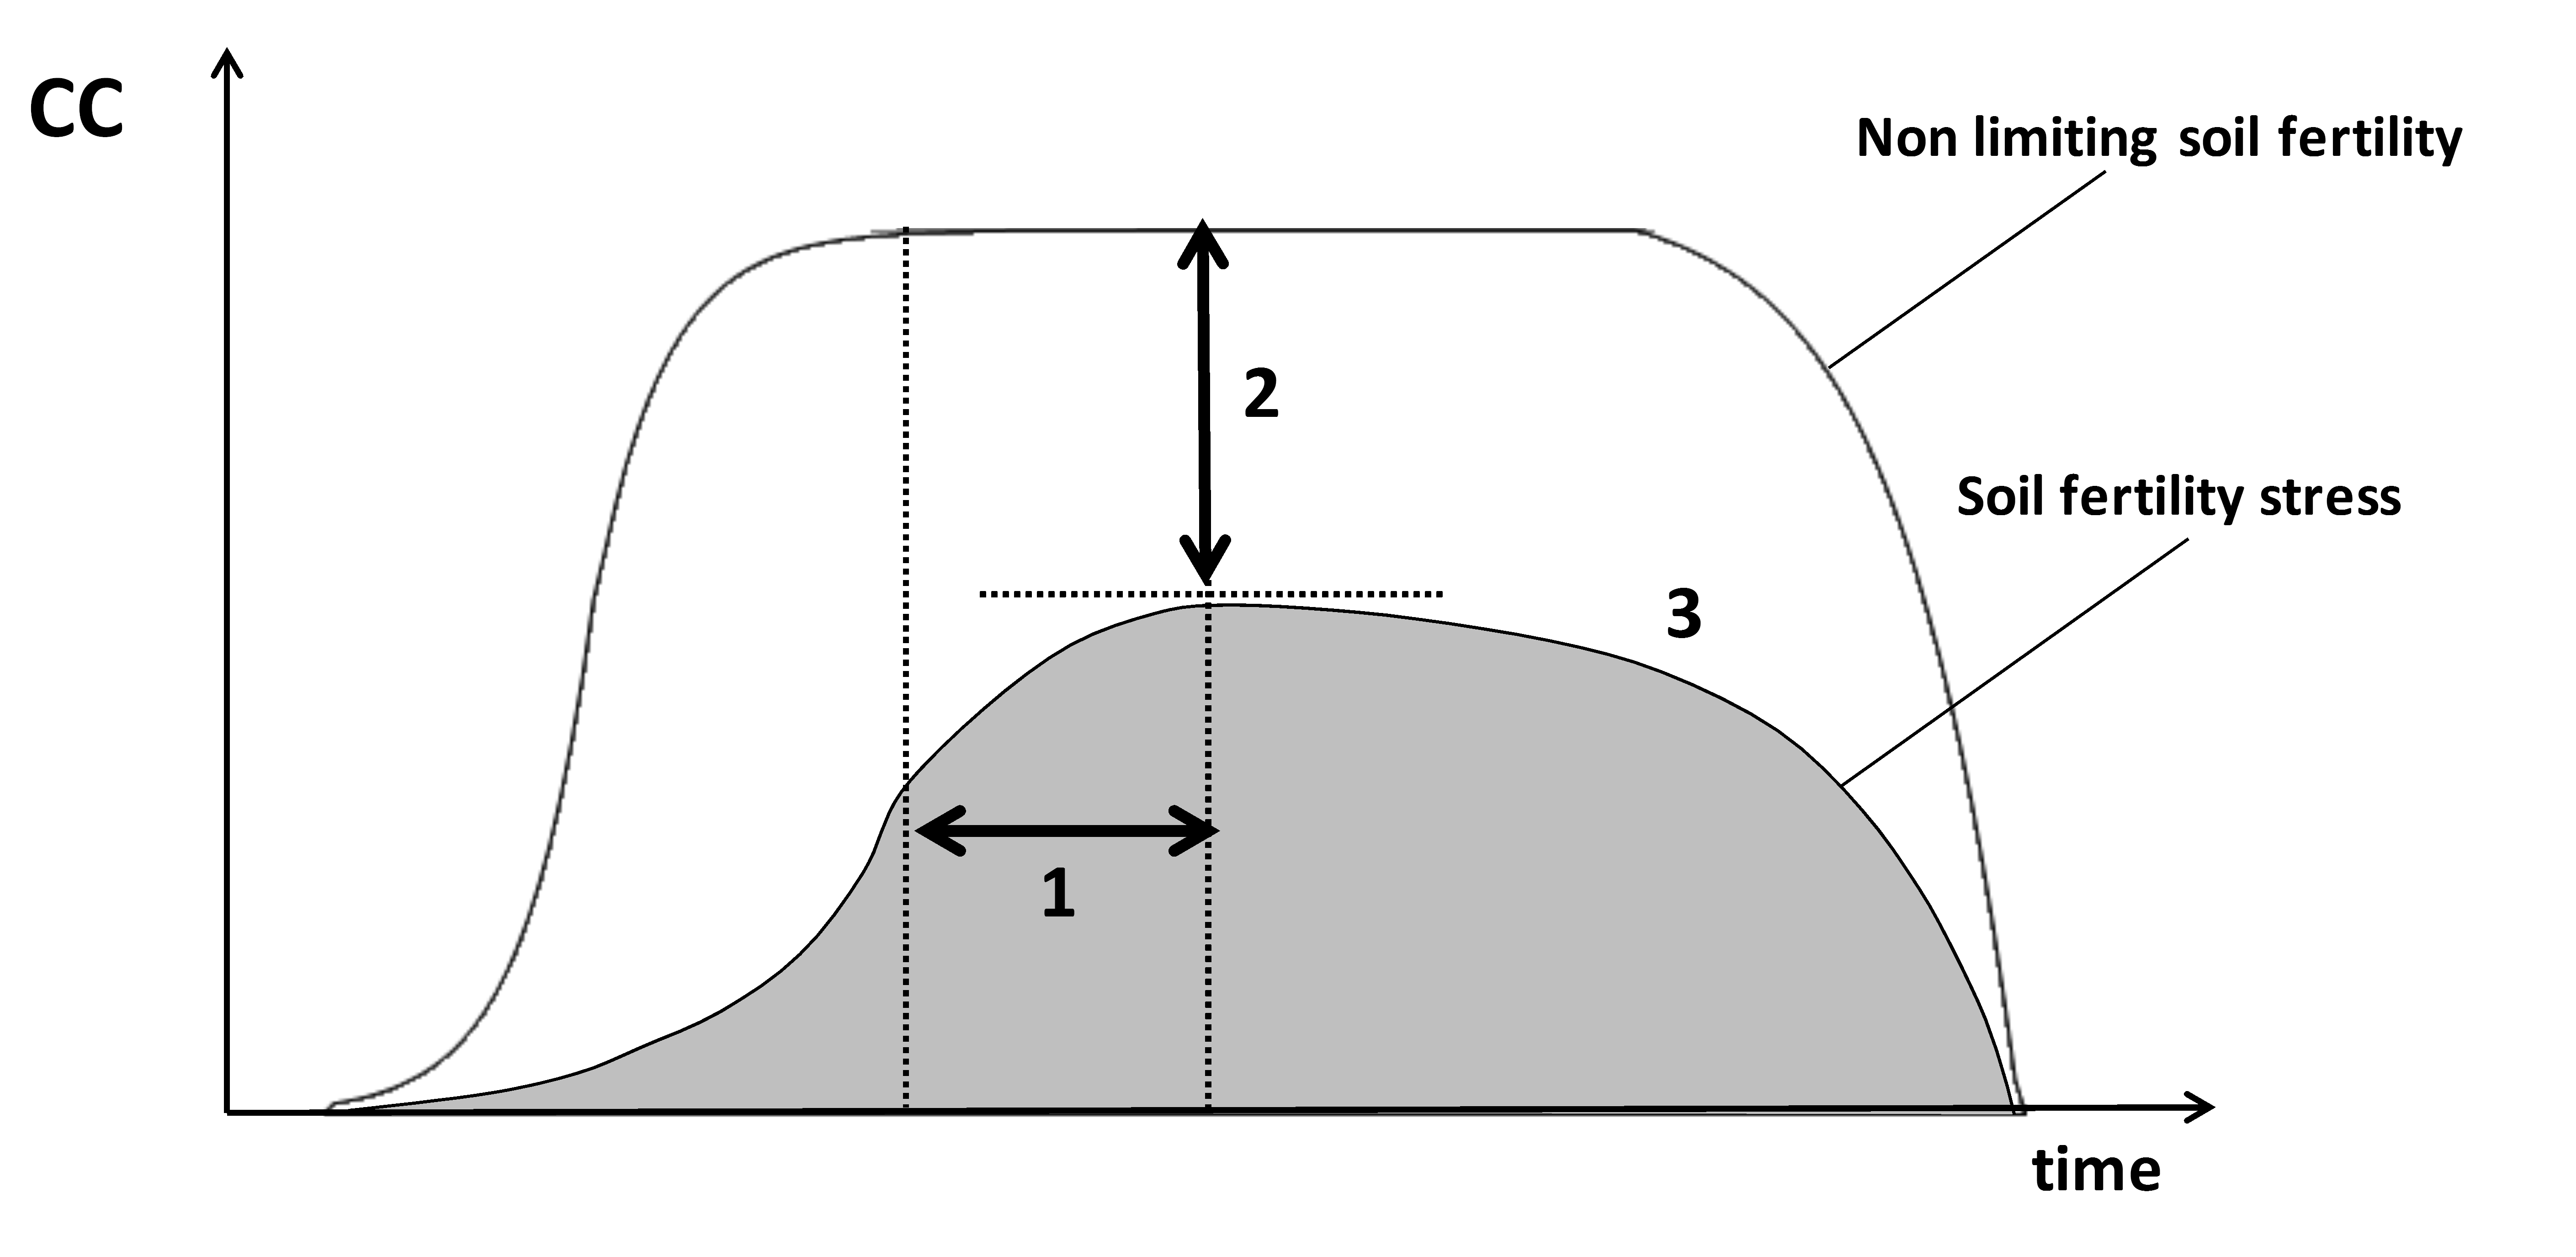
\includegraphics[width=12cm]{CCTheory_600dpi.png}
	\caption{Soil fertility stress affects green canopy cover (CC) development by means of (1) a slower canopy development, (2) a less dense canopy and (3) a steady decline in canopy cover once the maximum is reached during mid-season.}
	\label{fig:ch3_CCTheory}
\end{figure}

\begin{figure}[tbhp]
	\centering
		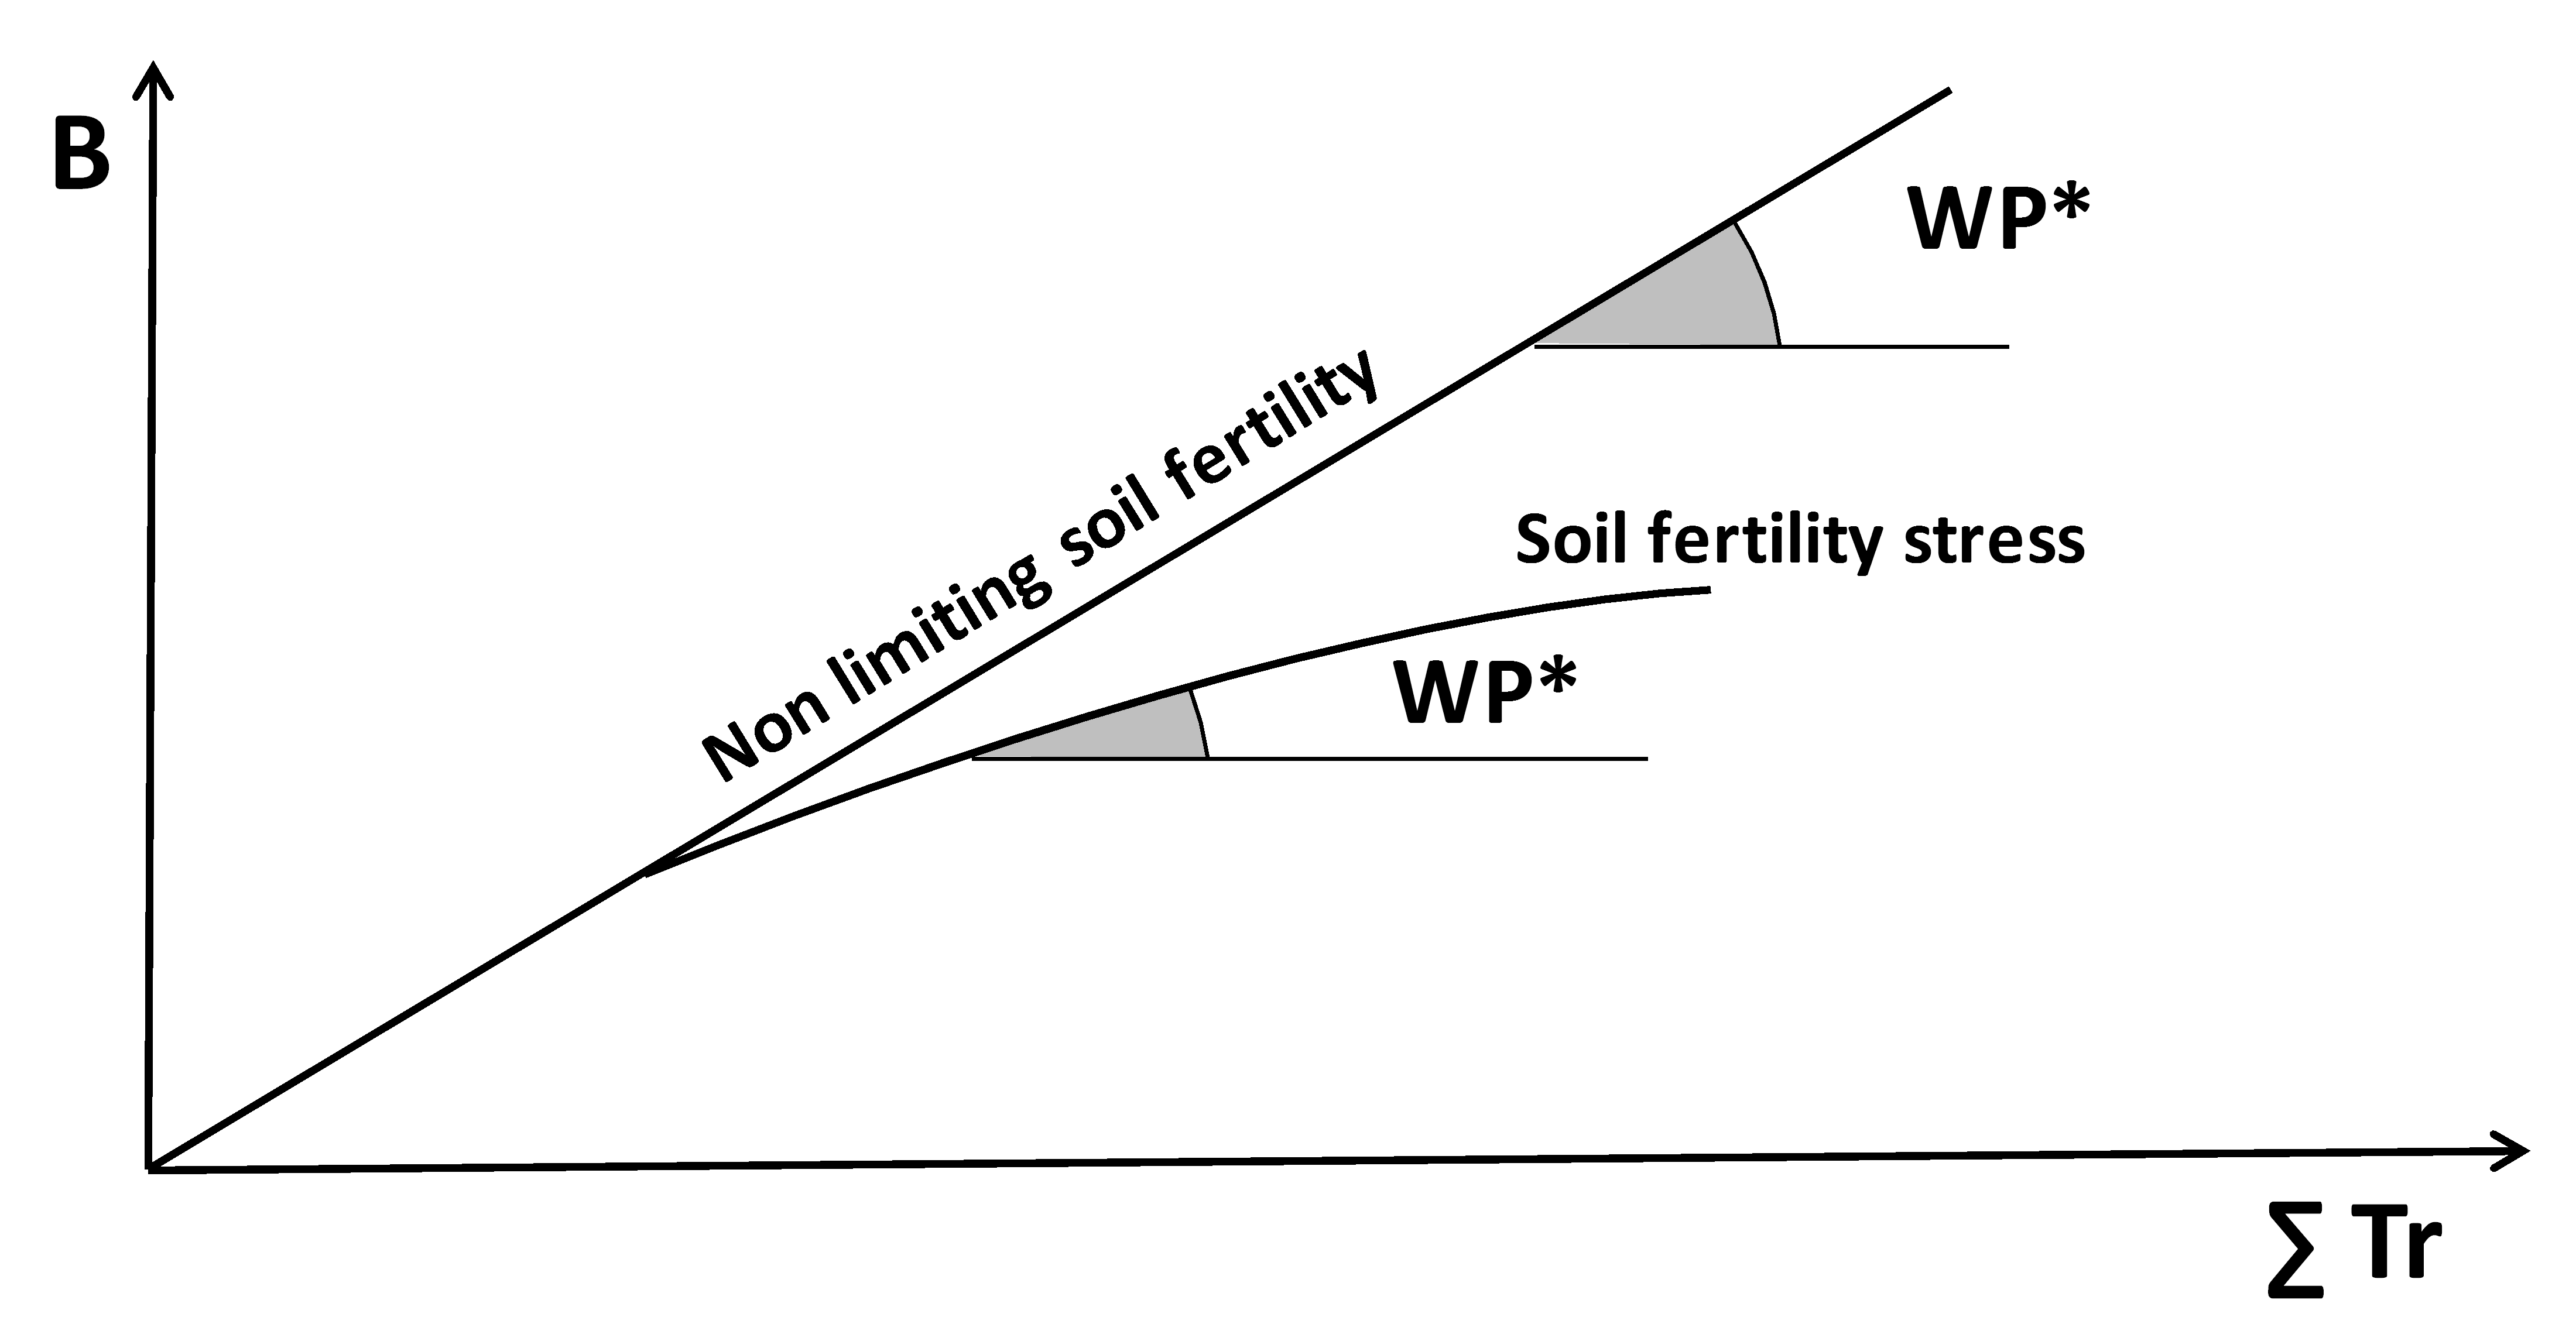
\includegraphics[width=12cm]{BTheory_600dpi.png}
	\caption{Soil fertility stress reduces biomass water productivity (\WPster) throughout the season as cumulative biomass (B) increases and the soil nutrient reservoir becomes depleted. The x-axis representing cumulative daily transpiration ($\Sigma Tr$) could also been seen as an axis representing time.}
	\label{fig:ch3_BTheory}
\end{figure}

To simulate these four crop responses to soil fertility stress, AquaCrop uses four stress coefficients, i.e. for canopy expansion ($Ks_{exp,f}$), for maximum canopy cover ($Ks_{CC_{x}}$), for biomass water productivity ($Ks_{WP}$) and for canopy decline ($f_{CDecline}$). As for water stress, stress coefficients range from 1 (no stress) to 0 (full stress). For every stress coefficient, a stress curve (\autoref{fig:ch3_stresscurve}(a)) defines the relationship between the level of soil fertility stress and the reduction of the target crop parameter (CGC, \CCx, \WPster and CC, respectively) that is affected by soil fertility stress. The shape of the stress curve can be convex, concave or linear, according to the position of the curve's calibration point (\autoref{fig:ch3_stresscurve}(a)). The calibration point is determined for each case through calibration of the parameters of the model. As mentioned above, even though the fertility stress simulation procedure is the same for different crops, the crop response to soil fertility is specific to the crop type and to the environmental conditions under which the crop is cultivated, including climate and soil type. Therefore, the crop response to soil fertility stress cannot be described using conservative crop parameters (independent of location, crop cultivar or management practice) but requires calibration for each case. 

To facilitate the calibration of the crop response to soil fertility stress, an automatic calibration procedure is incorporated in the latest AquaCrop software (version 4.0). This procedure requires field observations of \CCx and \Brel and a qualitative description of the observed canopy decline during the season for a `soil fertility stressed' calibration field in comparison to a `reference' field (no soil fertility stress). To avoid interference and interaction with other stress factors during calibration, both fields need to be free of soil water stress and salinity stress, as well as of diseases, weeds and pests. Based on the input of the field observations, the curves of the four soil fertility stress coefficients ($Ks_{exp,f}$, $Ks_{CC_{x}}$, $Ks_{WP}$ and $f_{CDecline}$), i.e. the soil fertility stress relationships (\autoref{fig:ch3_stresscurve}(a)), are automatically fixed by means of an iterative optimization algorithm. Next, the expected canopy development and reduction of biomass are calculated for every level of soil fertility stress between full stress and no stress, based on the four stress curves (\autoref{fig:ch3_stresscurve}(a)) and assuming no water stress. This results in the determination of the relative biomass-soil fertility stress relation (\autoref{fig:ch3_stresscurve}(b)). This relationship is not linear because (i) the shapes of the four stress curves are mostly non-linear, (ii) the shapes of the stress curves differ amongst the four stress coefficients, and (iii) the effect of soil fertility stress on \WPster increases when biomass increases. The AquaCrop reference manual version 4.0 \parencite{raes2012} contains more information about the automatic calibration procedure.

\begin{figure}[tbhp]
	\centering
		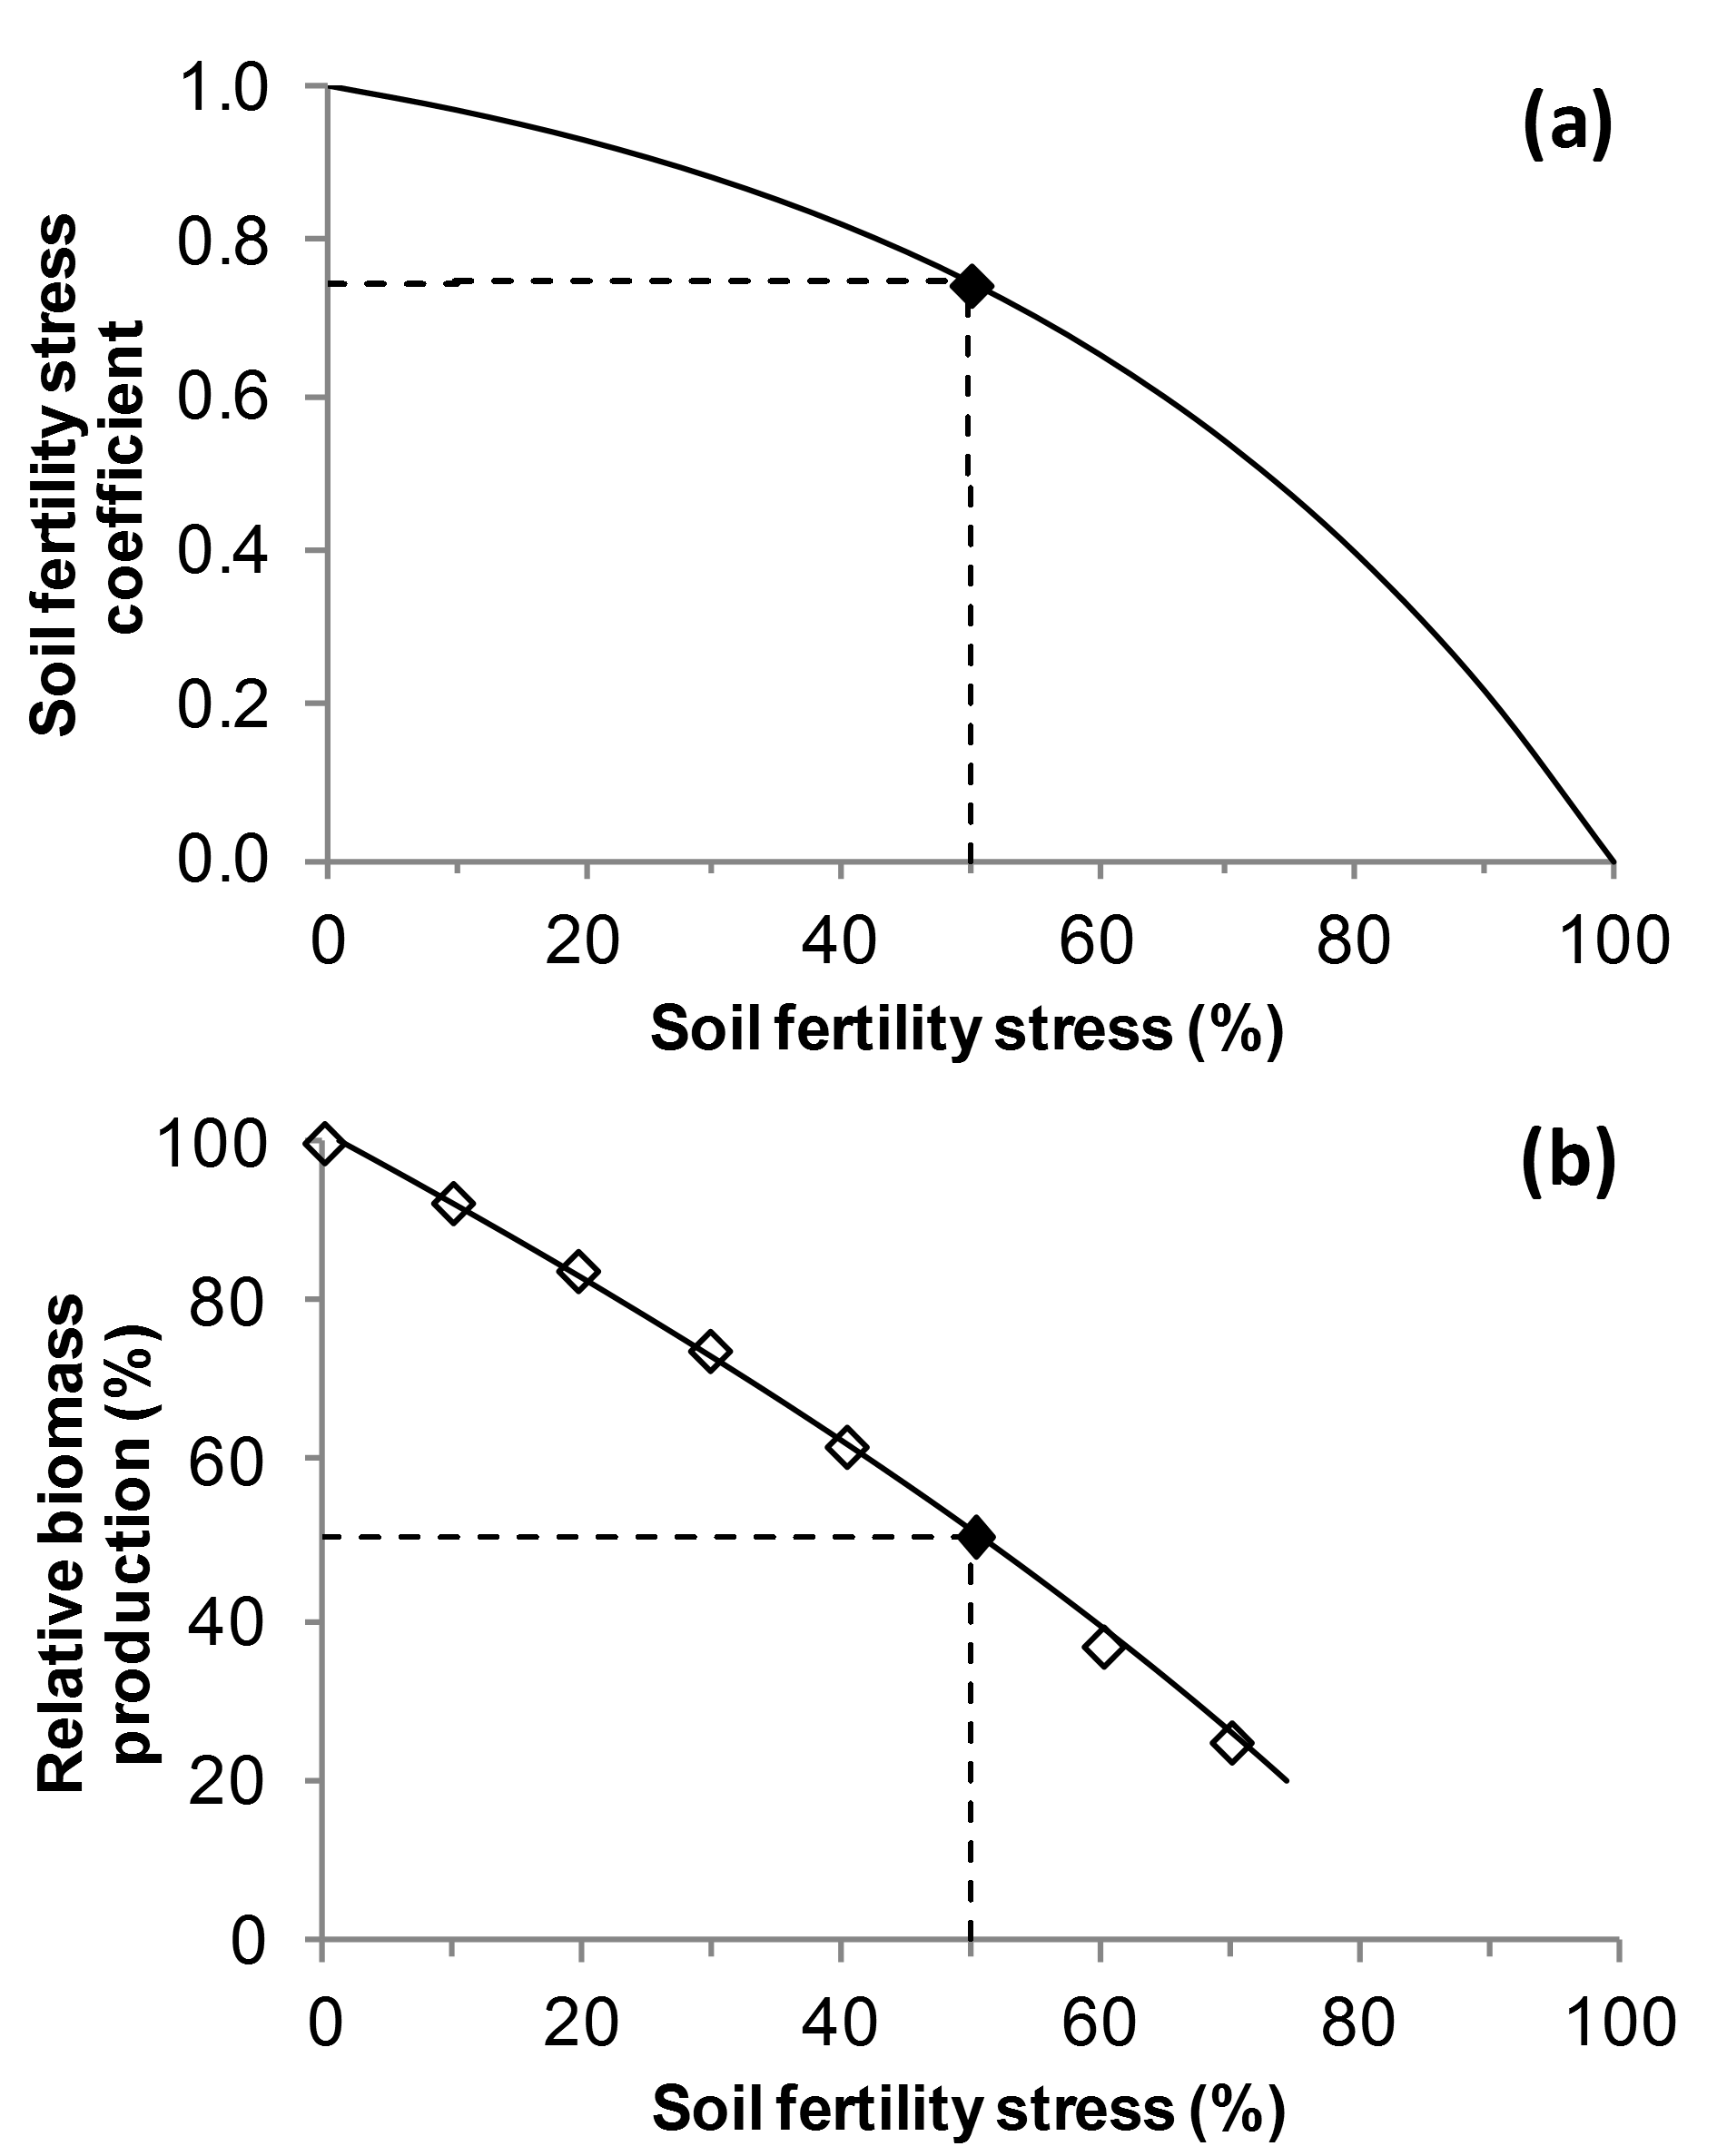
\includegraphics[height=12cm]{stresscurve_600dpi.png}
	\caption{Four stress curves of the type shown in (a), which represent the relationships between soil fertility stress and the four soil fertility stress coefficients, determine the relationship between relative biomass production (\Brel) and soil fertility stress (b). The calibration point (black point) determines the shape of a stress curve.}
	\label{fig:ch3_stresscurve}
\end{figure}

Once the crop response to soil fertility stress is calibrated, crop production can be simulated for specified soil fertility levels under various environmental and management conditions. In order to perform a simulation, the user needs to specify the soil fertility level in terms of \Brel (ranging from 20 to 100\%) or to select a class between `non-limiting' and `very poor' biomass production, which is linked to a default \Brel value. In the model, the user-specified input of \Brel is translated into a soil fertility stress level by means of the biomass – soil fertility stress relationship (\autoref{fig:ch3_stresscurve}(b)). Next, this soil fertility stress level is linked to the corresponding stress coefficients so that the four target parameters are adapted accordingly. Additionally, AquaCrop accounts for other stresses affecting biomass production by making a dynamic adjustment of the soil fertility stress level at every time step. If, for example, soil water stress limits biomass production during time step i, the simulated \Brel during time step i will be lower than the \Brel that would be expected during that time step on the basis of soil fertility stress alone ($B_{rel,input}$). Consequently, AquaCrop will reduce the soil fertility stress during time step i+1 in such a way that $B_{rel,input}$ could theoretically still be reached at the end of the crop cycle. This dynamic adjustment is justified because it can be assumed that the limitation of biomass production during time step i leaves more nutrients in the soil.

\subsection{Field experiments}
The semi-quantitative AquaCrop approach was tested against: (i) three years of experimental data for fields of tef (\textit{Eragrostis tef} (Zucc.) Trotter) in the drought-prone degraded highlands of Tigray in northern Ethiopia, (ii) two years of experimental data for fields of maize (\textit{Zea mays} L.) and wheat (\textit{Triticum aestivum} L.) in the humid plains of the central Terai in Nepal, and (iii) two years of experimental data for fields of quinoa (\textit{Chenopodium quinoa} Willd.)  in the semi-arid Bolivian Altiplano. \autoref{tab:ch3_metExp} presents a summary of the environmental conditions at the experimental sites. All experiments were set up with a (factorial) randomized complete block design, with the water treatment as main factor and the soil fertility treatment as sub-factor (\autoref{tab:ch3_metExp}). In rainfed (RF) and deficit irrigated (DI) treatments, some degree of water stress was apparent, whereas in the fully irrigated (IR) treatment crops were maintained free of any water stress. Fertility treatments corresponded to applications of 0\% (T0), 50\% (T50), 100\% (T100) and 150\% (T150) of the (national) recommended fertilizer dose (see \autoref{tab:ch3_metExp} for local recommendations). At all the experimental sites, the plots were regularly weeded and kept free from pests and diseases throughout the growing season. The following information was recorded: local daily weather data, soil water content in the root zone, the soil texture and physical characteristics, irrigation applications, fertilizer applications, crop development (green canopy cover development, monitored by overhead digital photographs), crop phenology (time of sowing, emergence, \CCx, flowering, senescence and maturity), effective rooting depth, intermediate and the final dry above-ground biomass, and the final grain yield. More detailed information on the set-up and data collection for the field experiments is described by \textcite{tsegay2012} for Ethiopia, by \textcite{shrestha2013a} for Nepal, and by \textcite{geerts2008a} for Bolivia.

\begin{landscape}
\begin{table}[htbp]
  	\caption{Three experimental sites with the experimental set up and environmental conditions (average climatic 	conditions according to New\_LocClim \parencite{fao2005}). Experiments were set up with a randomized complete block design (RCBD) or a factorial randomized complete block design (FRCBD). Water treatments consist of rainfed (RF), deficit irrigation (DI) and full irrigation (IR). Fertility treatments correspond to application of 0\% (T0), 50\% (T50), 100\% (T100) and 150\% (T150) of the (national) recommended fertilizer dose.}
    \resizebox{\linewidth}{!}
		{
	\begin{threeparttable}
  	\centering
		\begin{tabular}{lrrrc}
\toprule
\textbf{Experimental site} & \multicolumn{1}{c}{\textbf{Dejen}} & \multicolumn{1}{c}{\textbf{Maiquiha}} & \multicolumn{1}{c}{\textbf{Chitwan}} & \textbf{Patacamaya} \\
\midrule
Country & \multicolumn{1}{c}{Ethiopia} & \multicolumn{1}{c}{Ethiopia} & \multicolumn{1}{c}{Nepal} & Bolivia \\
Coordinates & \multicolumn{1}{c}{13°20' N, 39°22' E} & \multicolumn{1}{c}{13°48' N, 39°27' E} & \multicolumn{1}{c}{27°36' N, 84°24' E} & 17°14' S, 67°55' W \\
Altitude (m a.s.l.) & \multicolumn{1}{c}{2128} & \multicolumn{1}{c}{2078} & \multicolumn{1}{c}{160} & 3793 \\
\midrule
\multicolumn{2}{l}{\textbf{Environmental conditions}} &       &       &  \\
Soil type & \multicolumn{1}{c}{Loam, silty loam, sandy loam} & \multicolumn{1}{c}{Silty loam} & \multicolumn{1}{c}{Sandy loam} & Silty loam \\
Aridity & \multicolumn{1}{c}{Semi-arid} & \multicolumn{1}{c}{Semi-arid} & \multicolumn{1}{c}{Humid} & Semi-arid \\
Mean annual rainfall (mm) & \multicolumn{1}{c}{620} & \multicolumn{1}{c}{620} & \multicolumn{1}{c}{1870} & 403 \\
Mean annual ET0 (mm) & \multicolumn{1}{c}{1497} & \multicolumn{1}{c}{1497} & \multicolumn{1}{c}{1219} & 1208 \\
\midrule
\multicolumn{2}{l}{\textbf{Experimental set up}} &       &       &  \\
Years & \multicolumn{1}{c}{2008-2010} & \multicolumn{1}{c}{2009} & \multicolumn{1}{c}{2009-2011} & 2006/07 2009/10 \\
Number of seasons & \multicolumn{1}{c}{3} & \multicolumn{1}{c}{1} & \multicolumn{1}{c}{2} & 2 \\
Design & \multicolumn{1}{c}{FRCBD} & \multicolumn{1}{c}{FRCBD} & \multicolumn{1}{c}{RCBD/ FRCBD} & FRCBD \\
Crops & \multicolumn{1}{c}{tef} & \multicolumn{1}{c}{tef} & \multicolumn{1}{c}{wheat, maize} & quinoa \\
Water treatments$^{*}$ & \multicolumn{1}{c}{RF, IR} & \multicolumn{1}{c}{RF, IR} & \multicolumn{1}{c}{RF, DI, IR} & RF, DI, IR \\
Fertility treatments$^{**}$ & \multicolumn{1}{c}{T0, T50, T100} & \multicolumn{1}{c}{T0, T50, T100} & \multicolumn{1}{c}{T0, T100, T150} & T0, T50, T100 \\
\bottomrule				
    	\end{tabular}%
    	\begin{tablenotes}
    	%\vspace{0.05cm}
        \tiny{
      	\item[$\ast$] Various levels of water stress
      	\begin{itemize}
          \item[] RF: Rainfed, i.e. no supplementary irrigation
      	  \item[] DI: Deficit irrigation, i.e. treatment with partial irrigation: water stress is allowed during some parts of the crop cycle  
          \item[] IR: Full irrigation, i.e. kept free from any water stress   	
		\end{itemize}
		\item[$\ast\ast$] T0, T50, T100, T150: Application of 0\%, 50\%, 100\% and 150\% of the (national) recommended fertilizer dose 
		\begin{itemize}
        \item[] T100 tef: 60 kg/ha N and 26 kg/ha P on heavy soils and 40 kg/ha N and 26 kg/ha P on light soil  \parencite{earo2002}
		\item[] T100 maize: 120 kg/ha N, 60 kg/ha P, 40 kg/ha K \parencite{moac2010} 
		\item[] T100 wheat: 100 kg/ha N, 50 kg/ha P, 25 kg/ha K \parencite{moac2010} 
		\item[] T100 quinoa: 30 Mg/ha organic fertilizer (sheep manure) \parencite{miranda2012a}
		\end{itemize} 
		} 
    	\end{tablenotes}
        \end{threeparttable}
              }
  \label{tab:ch3_metExp}%
\end{table}%
\end{landscape}

\subsection{Calibration and evaluation of the semi-quantitative AquaCrop procedure}
As a starting point for the calibration of crop responses to soil fertility stress, the default crop parameters of AquaCrop version 4.0 \parencite{raes2012} were used for all four crops. The non-conservative cultivar-specific crop parameters, describing the crop phenology, were fine-tuned to match the local cultivar and environmental conditions. The resulting crop files described canopy development, biomass production and yield under both optimal agronomic conditions and water stress, but not at this stage the crop responses to soil fertility stress.

The crop response to soil fertility stress was calibrated based on field observations during the rainy season of 2010 for tef, during the dry season of 2010/11 for maize and wheat, and during the growing season of 2009/10 for quinoa. Tef was only calibrated for one of the experimental sites (Dejen), because it was assumed that the soil fertility and environmental conditions for both sites would be similar, and that the crop would therefore respond identically to soil fertility stress at both sites. In the automatic calibration procedure (\autoref{tab:ch3_metCalib}), observations of canopy cover development and of biomass for plots not experiencing water stress but undergoing full soil fertility stress (IR-T0) were compared to observations for plots undergoing neither water stress nor fertility stress (IR-T100 for Ethiopia and Bolivia and IR-T150 for Nepal). For the tef and quinoa experiments, the (national) recommended fertilizer dose (T100) was taken as the `reference', because the T100 treatment relieved crops from fertility stress. In contrast, T100 cannot represent non-limiting soil fertility for the maize and wheat experiments in Nepal, because production increases for maize and wheat were observed with fertilizer doses that exceeded the national recommended dose. For this reason, T150 was used as the reference for the calibration of the maize and wheat responses to soil fertility stress in Nepal. 


\begin{table}[htbp]
  \centering
  \caption{The relative dry above-ground biomass production (\Brel), maximum canopy cover (\CCx) and canopy decline in the season as observed for the soil fertility stressed calibration plots (IR-T0) of tef, maize, wheat and quinoa together with the resulting calibrated local effect of soil fertility stress on canopy development (canopy growth coefficient CGC, \CCx, canopy decline) and biomass water productivity (\WPster).}
    \resizebox{\textwidth}{!}
		{
    \begin{tabular}{llrrrrr}
	\toprule
	\multicolumn{2}{l}{\textbf{Crop}} & \multicolumn{1}{c}{Tef} & \multicolumn{1}{c}{Maize} & \multicolumn{1}{c}      {Wheat} & \multicolumn{1}{c}{Quinoa} \\
	\multicolumn{2}{l}{\textbf{Calibration location }} & \multicolumn{1}{c}{Dejen} & \multicolumn{1}{c}{Chitwan} & \multicolumn{1}{c}{Chitwan} & \multicolumn{1}{c}{Patacamaya} \\
    \midrule
	\multicolumn{2}{l}{\textbf{Input for calibration}} &       &       &       &  \\
	\Brel  & \multicolumn{1}{c}{(\%)} & \multicolumn{1}{c}{66} & \multicolumn{1}{c}{53} & \multicolumn{1}{c}{44} & \multicolumn{1}{c}{50} \\
	\CCx under soil fertility stress  & \multicolumn{1}{c}{(\%)} & \multicolumn{1}{c}{66} & \multicolumn{1}{c}{52} & \multicolumn{1}{c}{50} & \multicolumn{1}{c}{44} \\
	Canopy decline & \multicolumn{1}{c}{(-)} & \multicolumn{1}{c}{medium} & \multicolumn{1}{c}{medium} & \multicolumn{1}{c}{medium} & \multicolumn{1}{c}{medium} \\
   \midrule
	\multicolumn{2}{l}{\textbf{Results of calibration}} &       &       &       &  \\
	CGC reduction & \multicolumn{1}{c}{(\%)} & \multicolumn{1}{c}{15} & \multicolumn{1}{c}{15} & \multicolumn{1}{c}{39} & \multicolumn{1}{c}{36} \\
	\CCx reduction & \multicolumn{1}{c}{(\%)} & \multicolumn{1}{c}{19} & \multicolumn{1}{c}{31} & \multicolumn{1}{c}{44} & \multicolumn{1}{c}{41} \\
	Average canopy decline & \multicolumn{1}{c}{(\%/day)} & \multicolumn{1}{c}{0.78} & \multicolumn{1}{c}{0.85} & \multicolumn{1}{c}{0.28} & \multicolumn{1}{c}{0.19} \\
	\WPster reduction & \multicolumn{1}{c}{(\%)} & \multicolumn{1}{c}{19} & \multicolumn{1}{c}{31} & \multicolumn{1}{c}{50} & \multicolumn{1}{c}{19} \\
	\bottomrule
    \end{tabular}%
    }
  \label{tab:ch3_metCalib}%
\end{table}%

The calibrated crop response to soil fertility stress for each crop (\autoref{tab:ch3_metCalib}) was evaluated with the remaining, independent field datasets covering the different experimental sites (for tef), the different growing seasons, and the various water and fertility treatments. The observed \Brel for the non-water stressed treatments was used as input, but no alterations to the calibrated crop responses (\autoref{tab:ch3_metCalib}) were made; thus the biomass – soil fertility stress relation (\autoref{fig:ch3_stresscurve}(b)) was applied as described in the calculation procedure above. For both calibration and evaluation, the environmental conditions at the experimental sites were used as the inputs for the AquaCrop model. 
The fit between the observed and simulated soil water content, canopy cover, biomass and yield was assessed by a combination of graphical displays (plots of simulated versus observed values) and two statistical indicators, i.e. the relative root-mean-square error \parencite[RRMSE; \autoref{eq:ch3_RRMSE};][]{loague1991} and the coefficient of determination, or squared Pearson’s correlation coefficient \Rsq (\autoref{eq:ch3_Rsq}). In addition, the statistical significance of the Pearson’s correlation (R) between the observed and the simulated values was reported.

\begin{equation}
 RRMSE=RMSE \cdot \frac{100}{\overline{O}}=\dfrac{\sqrt{\sum_{i=1}^n(O_{i}-P_{i})^2}}{n} \cdot \frac{100}{\overline{O}}
  \label{eq:ch3_RRMSE}
\end{equation}

\begin{equation}
 R^{2}=\left(\dfrac{\sum_{i=1}^n(O_{i}-\overline{O})(P_{i}-\overline{P})}
                   {\sqrt{\sum_{i=1}^n(O_{i}-\overline{O})^2}  \cdot \sqrt{\sum_{i=1}^n(P_{i}-\overline{P})^2 }}
 \right)
  \label{eq:ch3_Rsq}
\end{equation}

where $O_{i}$ are the observed values, $P_{i}$ are the predicted values, \=O is the mean of the observed values,\=P is the mean of the predicted values and n is the number of observations.

Following \textcite{jamieson1991}, the performance of the model was classified based on RRMSE values as excellent (RRMSE < 10\%), good (10\% < RRMSE < 20\%), fair (20\% < RRMSE < 30\%) and poor (RRMSE > 30\%). Special attention was paid to the performance of the model under conditions in which soil water stress coincided with soil fertility stress. For this purpose, the performance of the model was also evaluated using only the RF and DI plots.  

\section{Results}
This section discusses the performance of the model in simulating crop responses to soil fertility stress, with a focus on the RRMSE values because they give a clear indication of the mean deviation of the simulation results obtained using the model, compared to the actual observations. Additionally, \autoref{tab:ch3_resCalib} (calibration) and \autoref{tab:ch3_resValid} (evaluation) present the \Rsq  values, with indications of the significance of the correlation (P-value).

\subsection{Calibration of the crop responses to soil fertility stress}
Crops were calibrated for different local soil fertility stress conditions (\autoref{tab:ch3_metCalib}). Soil fertility stress in the calibration fields was the highest for wheat (\Brel 44\%) and the lowest for tef (\Brel 66\%), with maize and quinoa being intermediate (\Brel 50-53\%). The calibration results (\autoref{tab:ch3_metCalib}) clearly show how the four crops in their specific environments responded very differently to the local nutrient limitations. For example, a soil fertility level \Brel of about 50\% resulted in a greater reduction in \WPster and in canopy decline in maize than in quinoa. By contrast, the reduction in crop development and \CCx was greater in quinoa than in maize. The calibrated effect of soil fertility on CC and \WPster (\autoref{tab:ch3_metCalib}) resulted in an acceptable simulation of Wr and of the overall development of CC and B throughout the crop cycle for the soil fertility stressed calibration plots (IR-T0) (\autoref{tab:ch3_resCalib}). The model performed excellent in simulating Wr, with RRMSE values below 10\% for all crops. For CC and B, the model performance was more variable, with RRMSE values mostly above 10\%. The model predicted CC with a mean deviation of about 16\% for tef, but the deviation increased to 20-24\% for wheat and maize. CC predictions could not be evaluated for quinoa, due to a lack of observations. With a RRMSE value of about 9\%, the best prediction of B was obtained for maize, followed by tef and wheat, for which RRMSE values were 12 and 14\% respectively. For quinoa, B was predicted with a RRMSE value of about 25\%. Generally, the model calibration was most accurate (based on the RRMSE values for Wr, CC and B) for maize and tef, followed by wheat and quinoa.

\begin{table}[htbp]
  \centering
  \caption{The relative root-mean-square error (RRMSE), coefficient of determination (\Rsq) and P-value for the Pearson’s correlation (R) for the soil water content in the root zone (Wr), canopy cover (CC) and dry above-ground biomass (B) during the growing season of the soil fertility stressed calibration plots (IR-T0). N is the number of sampled treatments during the season from those calibration plots.}
    %\resizebox{\textwidth}{!}
		%{
\begin{tabular}{rrccccc}
\toprule
\multicolumn{1}{l}{\textbf{Parameter}} &       &       & Tef   & Maize & Wheat & Quinoa \\
\midrule
\multicolumn{1}{l}{Wr} & \multicolumn{1}{l}{n} & (-)   & 15    & 5     & 8     & 5 \\
      & \multicolumn{1}{l}{RRMSE} & (\%)  & 5.6   & 2.6   & 6.7   & 9.6 \\
      & \multicolumn{1}{l}{\Rsq} & (-)   & 0.75  & 0.99  & 0.87  & 0.98 \\
      & \multicolumn{1}{l}{P-value} & (-)   & <0.01 & <0.01 & <0.01 & <0.01 \\
\midrule
\multicolumn{1}{l}{CC} & \multicolumn{1}{l}{n} & (-)   & 12    & 6     & 9     & - \\
      & \multicolumn{1}{l}{RRMSE} & (\%)  & 15.8  & 23.5  & 20.1  & - \\
      & \multicolumn{1}{l}{\Rsq} & (-)   & 0.97  & 0.91  & 0.87  & - \\
      & \multicolumn{1}{l}{P-value} & (-)   & <0.01 & <0.01 & <0.01 & - \\
\midrule
\multicolumn{1}{l}{B} & \multicolumn{1}{l}{n} & (-)   & 8     & 6     & 8     & 11 \\
      & \multicolumn{1}{l}{RRMSE} & (\%)  & 11.9  & 9.3   & 14.2  & 25.2 \\
      & \multicolumn{1}{l}{\Rsq} & (-)   & 0.96  & 1     & 0.95  & 0.97 \\
      & \multicolumn{1}{l}{P-value} & (-)   & <0.01 & <0.01 & <0.01 & <0.01 \\
\bottomrule
\end{tabular}%
    %}
  \label{tab:ch3_resCalib}%
\end{table}%

\subsection{Evaluation of crop responses to soil fertility stress}
The calibrated model performed well in simulating Wr, CC, B and Y for the remaining independent evaluation plots under different soil water stress levels (IR, DI and RF) and soil fertility stress levels (T0, T50 and T100 (only for Nepal)) (\autoref{tab:ch3_resValid}). The performance of the model in its simulation of CC was variable, with a RRMSE as high as 34\% for maize, although lower RRMSE values were obtained both for tef (23\%) and for wheat (12\%). For maize, this was probably a reflection of the relatively poor CC calibration (\autoref{tab:ch3_resCalib}), whereas for wheat it reflected the good CC calibration. Despite the CC predictions, Wr was the most accurately predicted of all the parameters, with RRMSE values of between 6 and 13\%. Together, the accuracy of the simulations of CC and Wr and the corresponding soil water stress levels determined the accuracy of prediction of B during the growing season and at maturity. \autoref{fig:ch3_BCC} illustrates that the effect of different soil fertility stress levels on the development of CC and B in a well-watered wheat field was well described by AquaCrop. The AquaCrop simulations clearly captured the slow canopy development, lower \CCx, early canopy decline and lower biomass production under different soil fertility levels as they were observed in the field. The development of B during the season, as well as the final value of B, was predicted most accurately for wheat, followed by maize; the final value of B was predicted with a RRMSE of only 4\% for wheat, and of 12\% for maize. For quinoa and tef, the mean deviations for the final B predictions were 18 and 24\%, respectively. Finally, Y was one of the most accurately predicted parameters, second only to Wr. For maize, the prediction of yield was excellent, with a RRSME of only 7\%. With RRMSE values of 10\% for wheat, 16\% for quinoa and 19\% for tef, the model resulted in good final Y predictions for all crops. This is also illustrated in Fig. 5. In general, the model performed most accurately (based on the RRMSE values) for maize (for which it produced the best predictions for Y and Wr) and wheat (for which it produced the best predictions for B and CC), followed by quinoa and by tef. 

\begin{table}[htbp]
  \centering
  \caption{The relative root-mean-square error (RRMSE), coefficient of determination (\Rsq) and P-value for the Pearson’s correlation (R) for the soil water content in the root zone (Wr), canopy cover (CC), dry above-ground biomass (B) during the season and at phenological maturity and the final grain yield (Y) of the evaluation plots with soil fertility stress (T0 and T50 for tef and quinoa, T0 and T100 for maize and wheat). The left-hand statistics include all water treatments (RF, DI and IR), while the right-hand statistics only include the plots with water stress (RF and DI). N is the number of sampled treatments during the season from the validation plots.}
    \resizebox{\textwidth}{!}
    {
\begin{tabular}{rrrccccccccc}
\toprule
      & \multicolumn{2}{r}{} &       & \multicolumn{4}{c}{All water treatments (RF, DI, IR)} & \multicolumn{4}{c}{Water stressed treatments (RF, DI)} \\
\multicolumn{3}{l}{\textbf{Parameter}} &       & Tef   & Maize & Wheat & Quinoa & Tef   & Maize & Wheat & Quinoa \\
\midrule
\multicolumn{2}{l}{Wr} & \multicolumn{1}{l}{n} & (-)   & 189   & 39    & 60    & 15    & 98    & 26    & 40    & 10 \\
\multicolumn{2}{r}{} & \multicolumn{1}{l}{RRMSE} & (\%)  & 11    & 5.8   & 9.4   & 13.3  & 12.2  & 6.5   & 10.1  & 16.5 \\
\multicolumn{2}{r}{} & \multicolumn{1}{l}{\Rsq} & (-)   & 0.9   & 0.89  & 0.9   & 0.93  & 0.9   & 0.91  & 0.91  & 0.89 \\
\multicolumn{2}{r}{} & P-value & (-)   & <0.01 & <0.01 & <0.01 & <0.01 & <0.01 & <0.01 & <0.01 & <0.01 \\
\midrule
\multicolumn{2}{l}{CC} & \multicolumn{1}{l}{n} & (-)   & 131   & 42    & 60    & -     & 65    & 28    & 49    & - \\
\multicolumn{2}{r}{} & \multicolumn{1}{l}{RRMSE} & (\%)  & 22.7  & 34.2  & 11.9  & -     & 26.8  & 38.1  & 12    & - \\
\multicolumn{2}{r}{} & \multicolumn{1}{l}{\Rsq} & (-)   & 0.92  & 0.82  & 0.95  & -     & 0.91  & 0.82  & 0.95  & - \\
\multicolumn{2}{r}{} & P-value & (-)   & <0.01 & <0.01 & <0.01 & -     & <0.01 & <0.01 & <0.01 & - \\
\midrule
\multicolumn{2}{l}{B} & \multicolumn{1}{l}{n} & (-)   & 96    & 39    & 51    & 43    & 50    & 26    & 34    & 30 \\
\multicolumn{2}{r}{} & \multicolumn{1}{l}{RRMSE} & (\%)  & 19.6  & 15.9  & 13.1  & 22.4  & 19.2  & 18.2  & 14.6  & 22.6 \\
\multicolumn{2}{r}{} & \multicolumn{1}{l}{\Rsq} & (-)   & 0.88  & 0.97  & 0.96  & 0.95  & 0.87  & 0.96  & 0.95  & 0.95 \\
\multicolumn{2}{r}{} & P-value & (-)   & <0.01 & <0.01 & <0.01 & <0.01 & <0.01 & <0.01 & <0.01 & <0.01 \\
\multicolumn{2}{l}{B at maturity} & \multicolumn{1}{l}{n} & (-)   & 15    & 6     & 6     & 13    & 8     & 4     & 4     & 10 \\
\multicolumn{2}{r}{} & \multicolumn{1}{l}{RRMSE} & (\%)  & 23.6  & 11.8  & 3.9   & 18.3  & 19.6  & 13.3  & 3.5   & 15.2 \\
\multicolumn{2}{r}{} & \multicolumn{1}{l}{\Rsq} & (-)   & 0.77  & 0.95  & 0.96  & 0.91  & 0.82  & 0.97  & 0.98  & 0.87 \\
\multicolumn{2}{r}{} & P-value & (-)   & <0.01 & <0.01 & <0.01 & <0.01 & <0.01 & <0.05 & <0.05 & <0.01 \\
\midrule
\multicolumn{2}{l}{Y} & \multicolumn{1}{l}{n} & (-)   & 15    & 6     & 6     & 13    & 8     & 4     & 4     & 10 \\
\multicolumn{2}{r}{} & \multicolumn{1}{l}{RRMSE} & (\%)  & 19.1  & 7.2   & 10.3  & 16.3  & 34    & 10.7  & 11.9  & 13 \\
\multicolumn{2}{r}{} & \multicolumn{1}{l}{\Rsq} & (-)   & 0.85  & 0.99  & 0.77  & 0.81  & 0.21  & 0.99  & 0.93  & 0.86 \\
\multicolumn{2}{r}{} & P-value & (-)   & <0.01 & <0.01 & <0.05 & <0.01 & NS    & <0.01 & <0.05 & <0.01 \\
\bottomrule
\end{tabular}%
    }
  \label{tab:ch3_resValid}%
\end{table}%


\begin{figure}[tbhp]
	\centering
		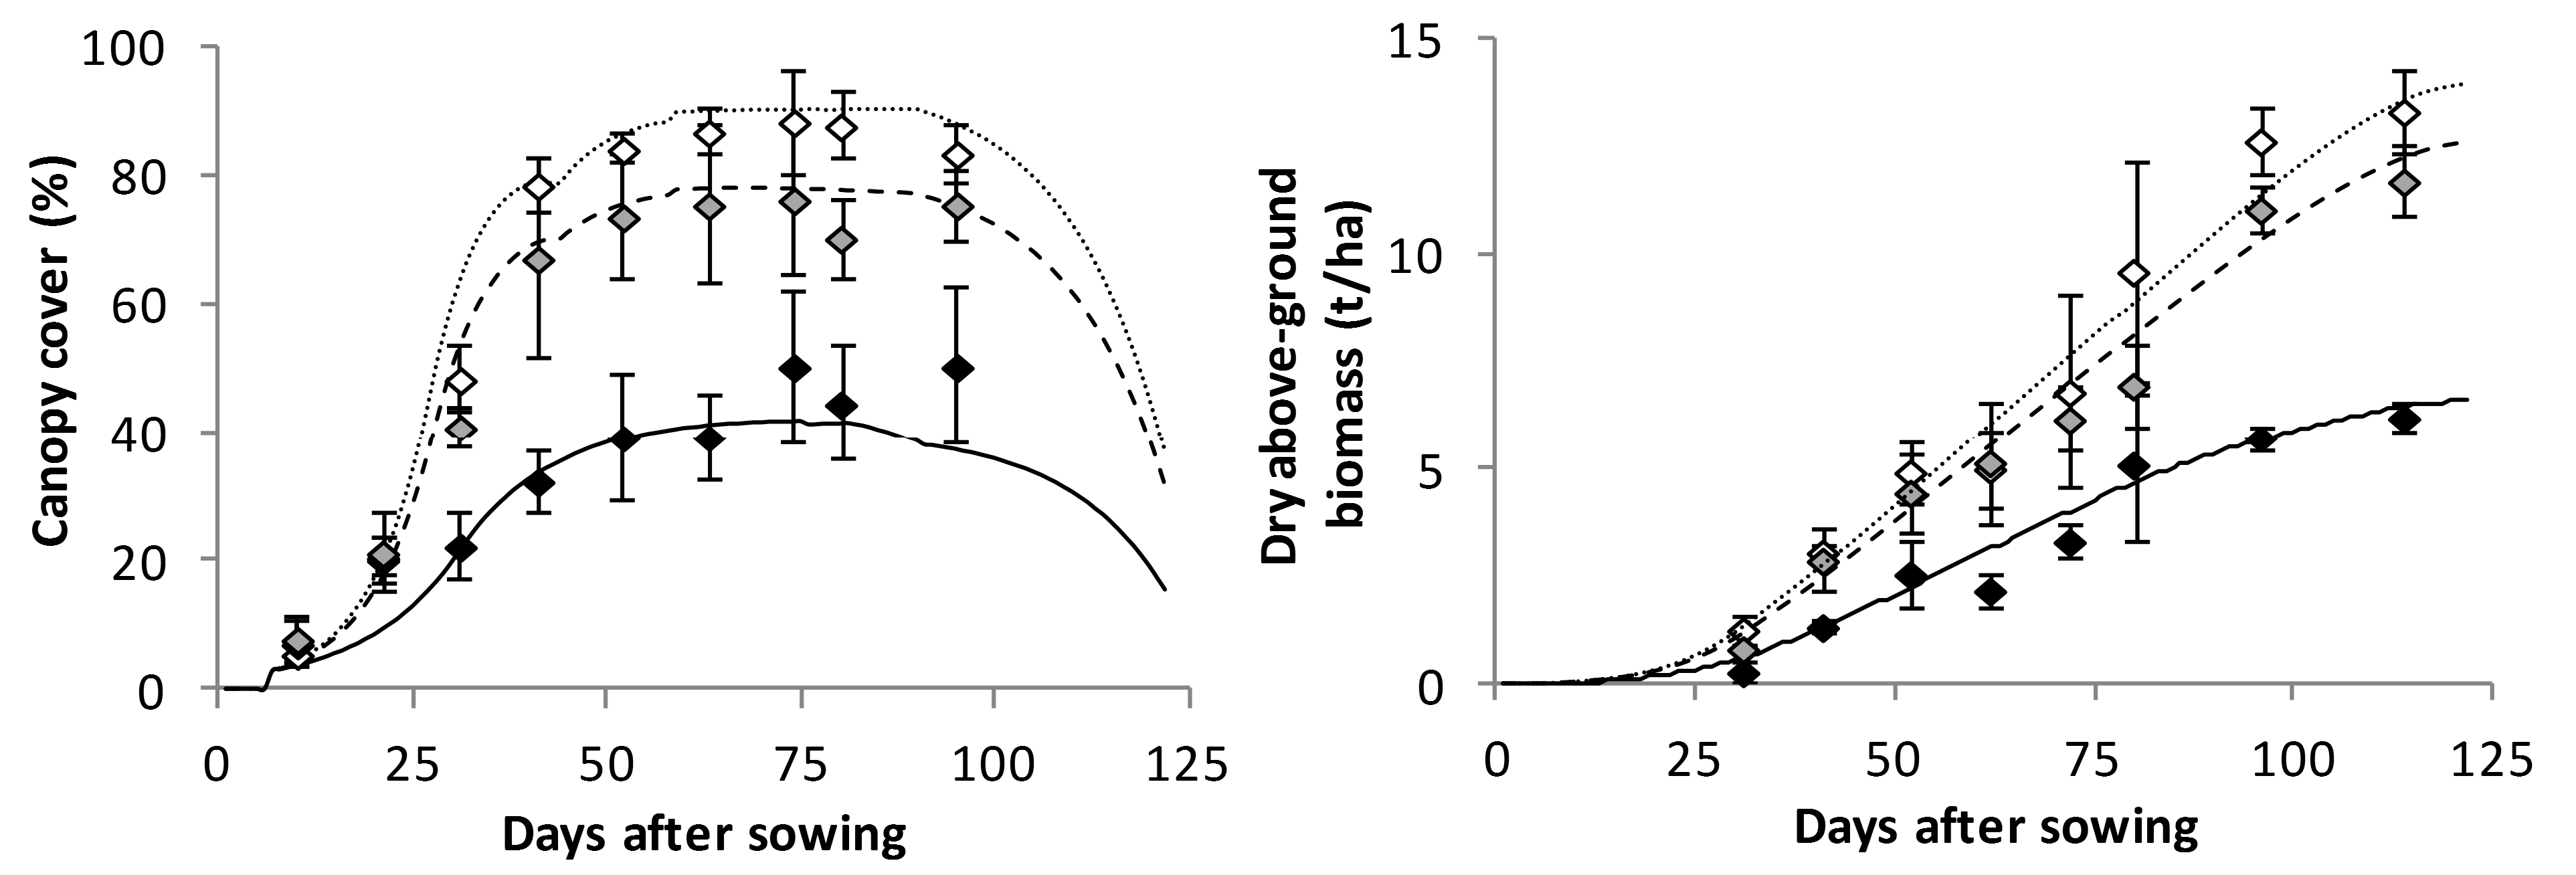
\includegraphics[width=12cm]{BCC_600dpi.png}
	\caption{Simulated (lines) and observed (symbols) canopy cover (left) and dry above-ground biomass (right) of irrigated wheat in Chitwan during the season of 2010/11. Canopy development and biomass build-up are affected by the soil fertility level: non-limiting soil fertility T150 (dotted line, open symbol), full soil fertility stress T0 (full line, black symbol), and fertility treatment with 100\% of the national recommended fertilizer dose T100 (dashed line, grey symbol). Error bars indicate $\pm$ standard deviation for three replications (n=3).}
	\label{fig:ch3_BCC}
\end{figure}

\begin{figure}[tbhp]
	\centering
		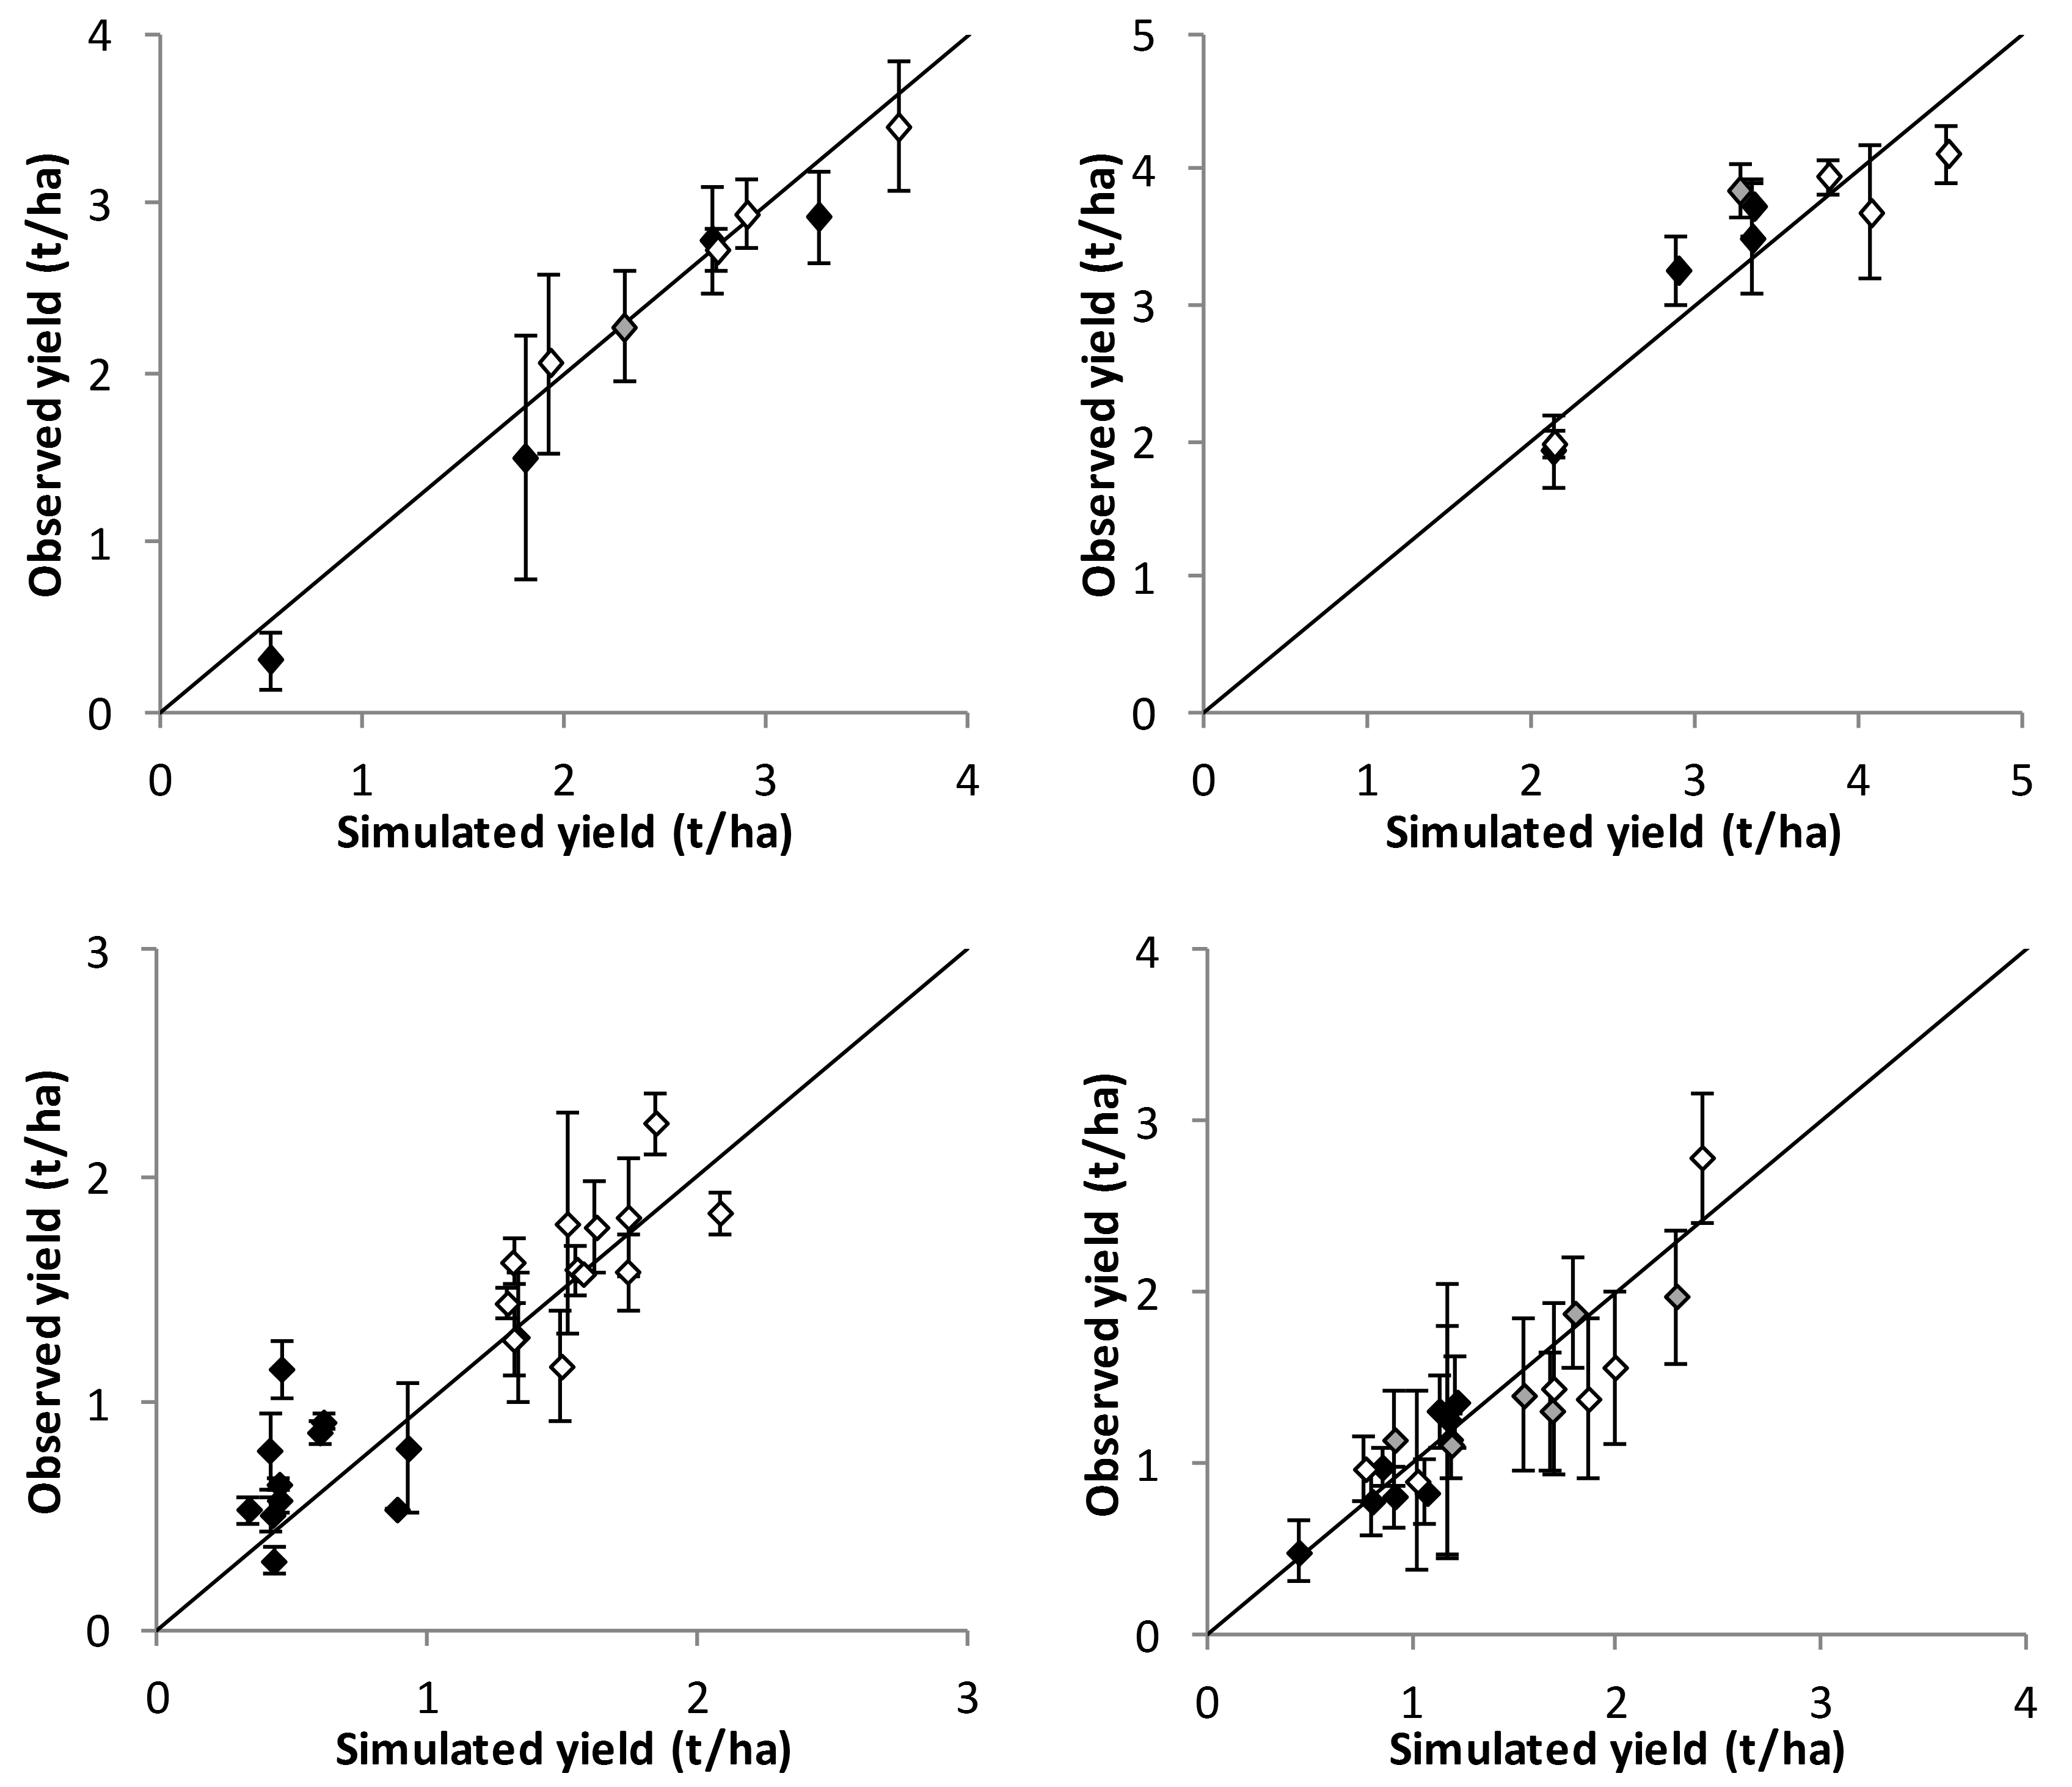
\includegraphics[width=12cm]{Yall_600dpi.png}
	\caption{Observed versus simulated yield for maize (top left) and wheat (top right) in Nepal, for tef in Ethiopia (bottom left) and for quinoa in Bolivia (bottom right) for all simulated environmental conditions, soil fertility levels (T0, T50, T100 and T150) and water treatments (IR white symbols, DI grey symbols and RF black symbols). Error bars indicate $\pm$ standard deviation for three replications (n=3).}
	\label{fig:ch3_Yall}
\end{figure}

\subsection{Performance of the model under combined soil fertility stress and water stress}
When both soil fertility stress and water stress were prevalent, AquaCrop was still able to predict the evolution of Wr (\autoref{fig:ch3_SWC}), CC (\autoref{fig:ch3_CC}) and B (\autoref{fig:ch3_B}) accurately during the growing season. The statistics for the water stressed plots only (DI and RF) in \autoref{tab:ch3_resValid} show that the fit is approximately as good as when all the water treatments (IR, DI and RF) are included. Compared to the evaluation for all the water treatments, the RRMSE values increased by only 0.7-3.2\% for Wr, 0.1-4\% for CC, and 0.2-2.3\% for B, for the water stressed plots alone. For B, in the cases of tef and quinoa, the performance of the model at maturity was even better when only the water stressed conditions were taken into account (RRMSE decreased by 3-4\%). The model predicted Y under combined water stress and soil fertility stress with a RRMSE of between 11 and 13\% for maize, wheat and quinoa. The deviation only increased by 1.6\% (wheat) and by 3.5\% (maize), and for quinoa it even decreased (by about 3\%). For tef, on the other hand, the predictions of Y under combined soil water stress and soil fertility stress were rather poor. The RRMSE was as high as 34\% and the correlation between the observed and the simulated values was insignificant. This may be due to inaccurate simulation of the effect of water stress on the harvest index. Finally, \autoref{fig:ch3_Yall} also shows how, with its semi-quantitative soil fertility approach, AquaCrop is able to predict values for grain production that range from as little as 0.5 t/ha to more than 4 t/ha as a result of the various climatic, agronomic and environmental conditions and from the combinations of soil fertility and soil water stress levels.

\begin{figure}[tbhp]
	\centering
		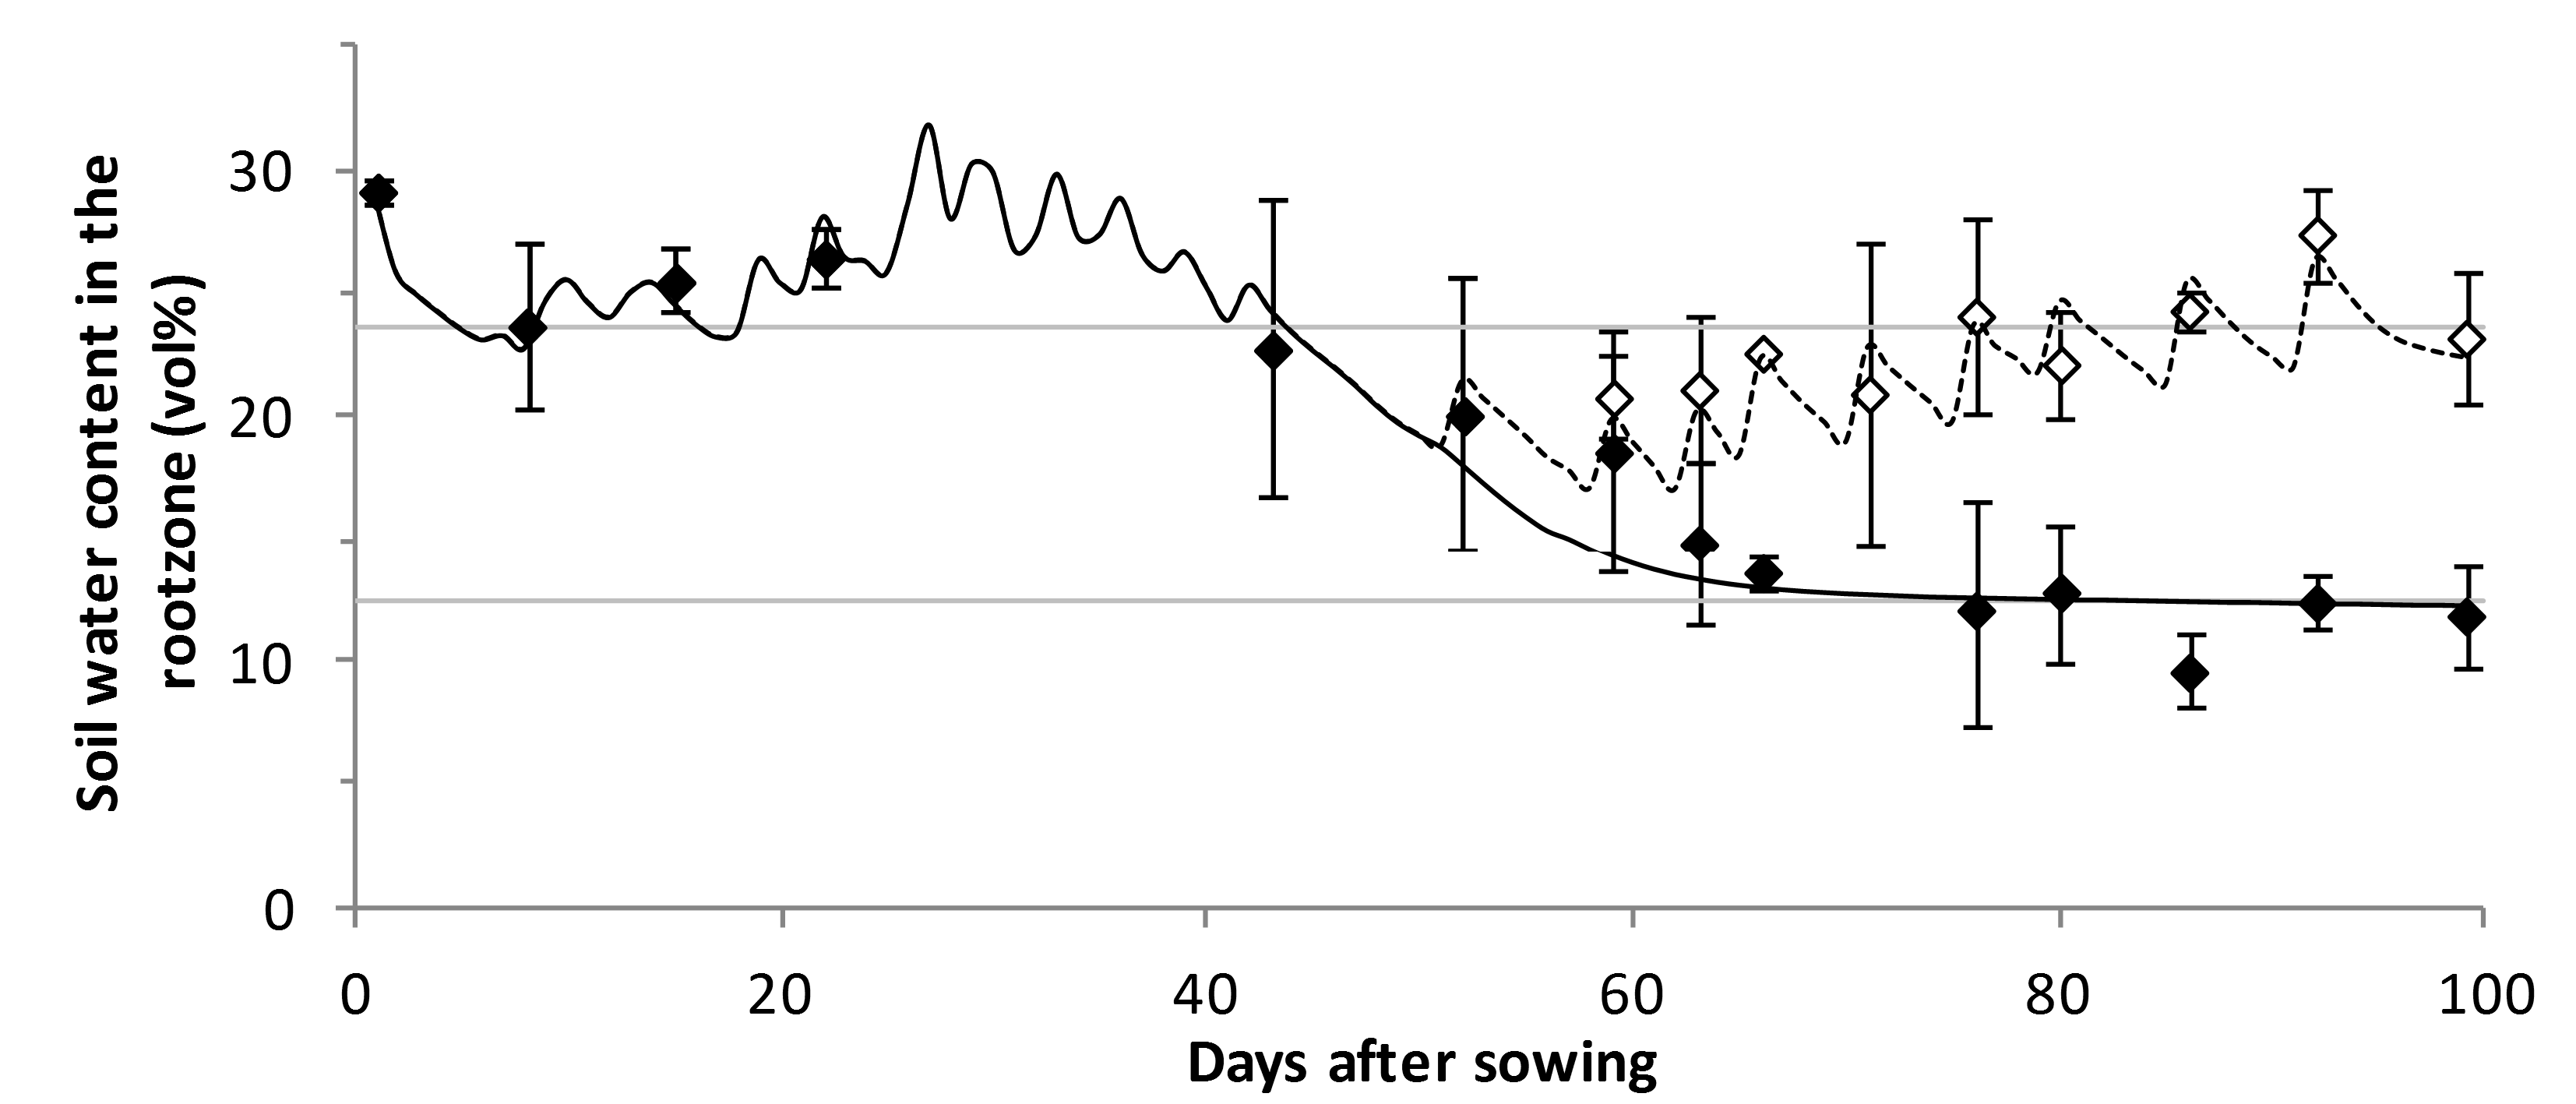
\includegraphics[height=5cm]{SWC_600dpi.png}
	\caption{Simulated (lines) and observed (symbols) soil water content in the root zone for tef under soil fertility stress (T50) in Dejen, during the season of 2010. Both irrigated (IR, dotted line, open symbol) and rainfed (RF, full line, filled symbol) soil water content are well simulated. Horizontal grey lines indicate the soil water content at field capacity (top line) and permanent wilting point (bottom line). Error bars indicate $\pm$ standard deviation for three replications (n=3).}
	\label{fig:ch3_SWC}
\end{figure}

\begin{figure}[tbhp]
	\centering
		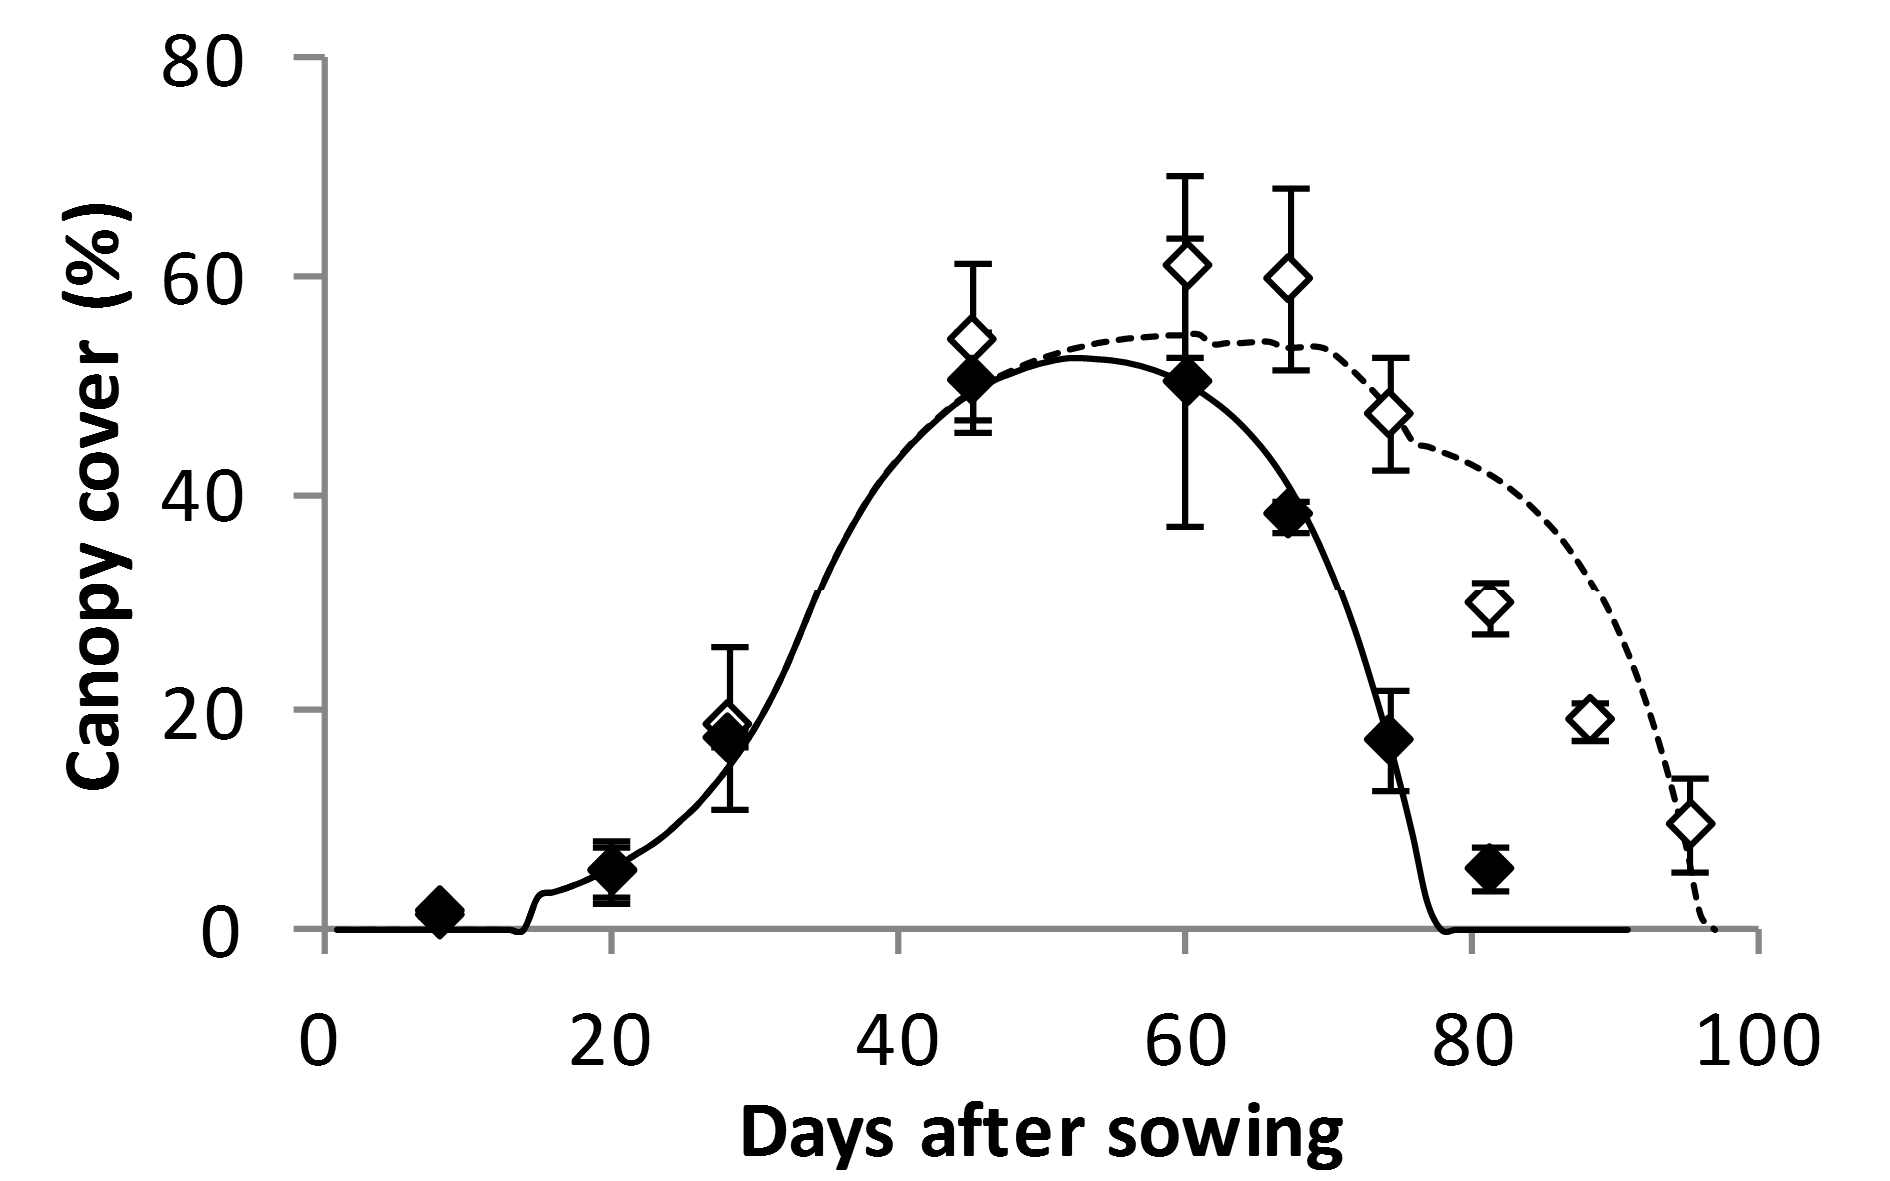
\includegraphics[height=5cm]{CC_600dpi.png}
	\caption{Simulated (lines) and observed (symbols) green canopy cover for tef under soil fertility stress (T0) in Maiquiha during the season of 2009. Both irrigated (IR, dotted line, open symbol) and rainfed (RF, full line, filled symbol) canopy cover development under soil fertility stress are well simulated. Error bars indicate $\pm$ standard deviation for three replications (n=3).}
	\label{fig:ch3_CC}
\end{figure}

\begin{figure}[tbhp]
	\centering
		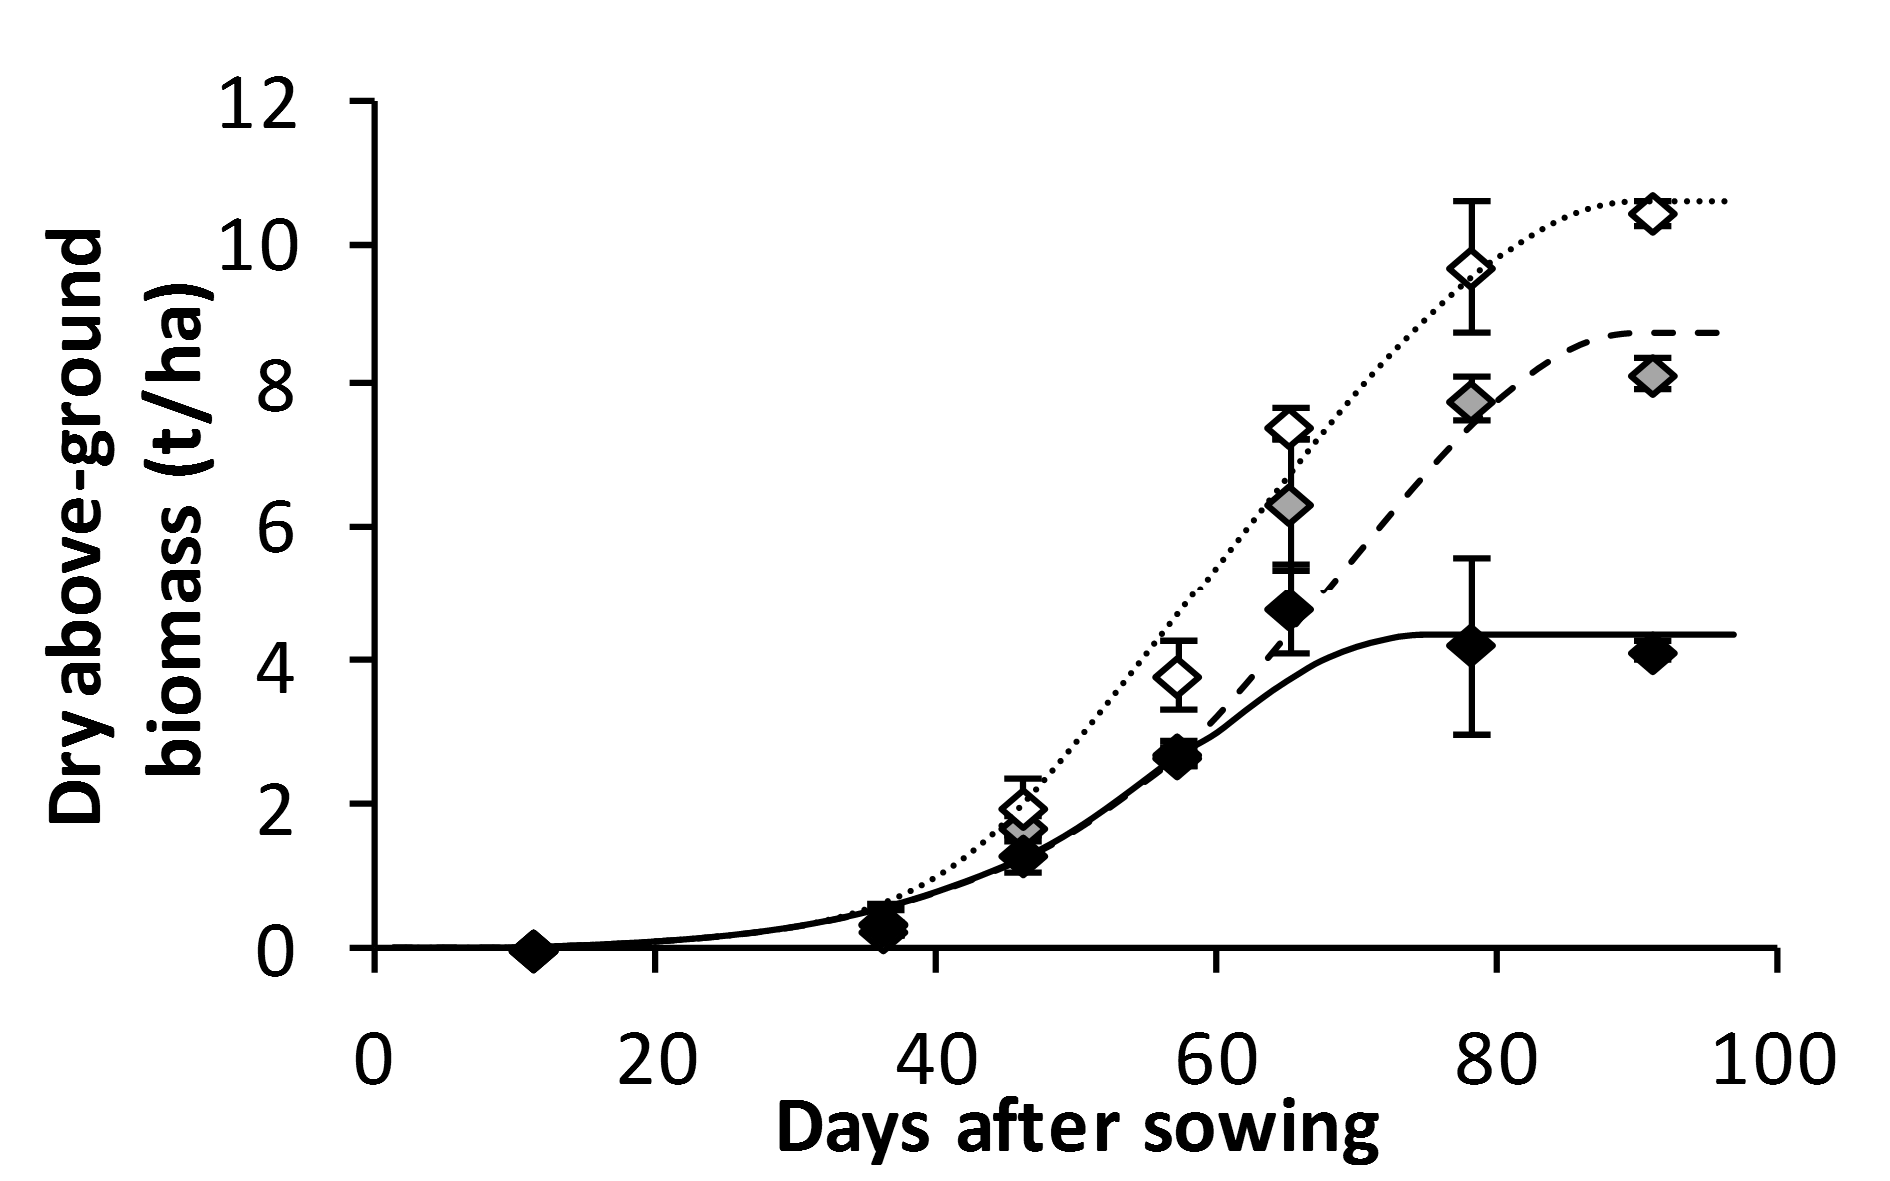
\includegraphics[height=5cm]{B_600dpi.png}
	\caption{Simulated (lines) and observed (symbols) dry above-ground biomass for maize in Chitwan during the season of 2009/10. Irrigated (IR, dotted line, open symbol), deficit irrigated (DI, dashed line, grey symbol) and rainfed (RF, full line, black symbol) biomass production under soil fertility stress (T100) are all well simulated. Error bars indicate $\pm$ standard deviation for three replications (n=3).}
	\label{fig:ch3_B}
\end{figure}

\section{Discussion}
\subsection{Performance of the semi-quantitative AquaCrop approach}
Because the semi-quantitative AquaCrop procedure uses the relative biomass of a fertility-stressed field compared to that of a reference field (\Brel) as the input from which to determine the soil fertility stress coefficients, it appears obvious that the final biomass, and consequently the yield simulations, for fertility stressed fields match the observations that are made in the absence of water stress. Nevertheless, the present study has shown that the semi-quantitative AquaCrop soil fertility procedure provides realistic results; not only were the final biomass and the yield simulated with acceptable accuracy (RRMSE of 4-24\% for B at maturity and 7-19\% for Y), but the soil water content, canopy cover and biomass development during the growing season were all also simulated with satisfactory accuracy (RRMSE of 6-13\% for Wr, 12-34\% for CC and 13-22\% for B) – and even for stress levels for which the model had not been calibrated. Moreover, it has been shown that AquaCrop can provide good indicative values for final biomass (RRMSE of 4-15\%) and for yield (RRMSE of 11-13\%) of maize, wheat and quinoa when crop production is affected by both soil fertility stress and soil water stress. In the case of tef, although biomass production was well simulated (RRMSE of 20\%) under conditions of combined soil water stress and soil fertility stress, yield predictions were poor (RRMSE of 34\%). Also \textcite{tsegay2012} noted, under conditions of non-limiting soil fertility, that AquaCrop performs less well in the estimation of tef yield under water-stressed conditions. Further calibration of the effects of water stress on the harvest index of tef might be necessary in order to improve yield predictions under water stressed conditions, both with and without soil fertility stress.

Notwithstanding its simplicity, the AquaCrop semi-quantitative approach performs as well as nutrient-balance-based models for the simulation of maize and wheat production under different levels of soil fertility stress and soil water stress. In evaluating simulations of wheat and maize production under different water and nitrogen treatments, \textcite{fang2008} found RRMSE values of 12\% for biomass and 12-15\% for yield with the CERES model, whereas \textcite{brisson2002} reported RRMSE values of 2-3\% for biomass but 16-24\% for yield using the STICS model; and \textcite{stockle2003} reported RRMSE values between 8 and 14\% for biomass and 8 and 32\% for yield simulated with the CropSyst model. The APSIM model has been evaluated on a number of occasions for the simulation of more challenging situations such as, for example, the response of a crop to phosphorus or organic fertilizer. \textcite{micheni2004} and \textcite{kinyangi2004} obtained \Rsq values of between 0.75 and 0.88 for the simulation of maize biomass production grown with organic fertilizer. Evaluating the simulation of maize production under different phosphorus and nitrogen supply levels, \textcite{fosumensah2012} found RRMSE values of about 15\% for yield and \Rsq values for biomass of between 0.89 and 0.91 (corresponding to RMSE values of 0.661 - 0.780 t/ha). Finally, \textcite{delve2009}, who studied the performance of maize grown under different phosphorus sources (manure versus fertilizer) and treatments (rate and frequency of application), found \Rsq values of 0.83-0.88 for biomass (corresponding to RRSME values of at least 26\%) and of 0.74-0.81 for yield. For maize and wheat, the performance statistics found in this study (\autoref{tab:ch3_resValid}) are clearly within the range of statistics reported for studies with nutrient-balance-based models. For tef and quinoa, the performance of the model cannot be compared to the performance of other crop models, since AquaCrop is currently the only crop model that has been calibrated to simulate crop production for these under-utilized crops \parencite{geerts2009, tsegay2012}.

It should also be noted that the present study evaluated the performance of AquaCrop’s fertility response algorithms against observations that were obtained from on-farm experiments in relatively small plots. As such, problems such as lodging of the crop, damage to some of the plots, (partial) loss of samples due to technical problems and transport, and a limited sample size during the growing season could not be avoided. This inevitably led to deviations among replicates that were sometimes substantial, and this led to large standard deviations in the graphs presented. It can be expected that similar experiments conducted in a controlled environment of an experimental research station would yield an even better match between the observed and simulated values for soil water balance, canopy development, biomass production and yield.

\subsection{Input and calibration requirements}
The semi-quantitative approach of AquaCrop requires the user to specify the soil fertility level, expressed as the relative biomass (\Brel) that can be expected in a fertility-stressed field compared to that for a reference field in non-water-stressed conditions. The \Brel can readily be obtained from farmers, from experimental fields or from agricultural statistics relating to local crop production. The ease with which this input can be obtained makes the semi-quantitative AquaCrop approach user-friendly and accessible to users worldwide. Moreover, the approach integrates the effects of various soil nutrients (and not merely nitrogen) and mineralization processes without a requirement for vast amounts of input data, for initialization of the soil nutrient conditions, or for elaborate parameterization.

The AquaCrop model is applicable to different crops and environmental conditions, but the crop response to soil fertility stress is crop- and case-specific and consequently the model requires calibration in each case. The necessity for a case-specific calibration diminishes the practicability of the model for analyses on a large spatial scale, but in this respect AquaCrop is no different from models that make use of a nutrient-balance approach, which also need site-specific information \parencite{gabrielle2002, matthews2002c}. Indeed, when crop production is being assessed over large areas, not only may various crops be being grown, but also the management, and the soil and nutrient conditions, may vary between different fields. Since each type of nutrient limitation affects canopy cover development and biomass in a different way, the crop response to soil fertility stress may differ amongst fields, even when the same crop is being grown. For example, a crop grown in a field where nitrogen is the most limiting nutrient will respond to the local soil fertility stress in a completely different way from a crop grown in a field where potassium is the most limiting nutrient. 
Fortunately, as this research shows, when simulations are run for different fields within the same area, in which the constraints on crop growth are similar, the calibrated crop response to soil fertility stress is quite robust. In the present study, for example, the response of tef to soil fertility stress was calibrated for one of the experimental sites (Dejen), but the model also performed well in simulating crop development and production at the other experimental site (Maiquiha). In another assessment using AquaCrop in Ethiopia, in which the barley yield gap was investigated at the district level, it was demonstrated that after calibrating the response of barley to soil fertility stress for one experimental site, AquaCrop could estimate with acceptable accuracy (\Rsq of 0.84 for B and 0.87 for Y, RMSE 0.82 t/ha for B and 0.23 t/ha for Y) barley biomass and yield under soil fertility stress for other farmers' fields within the same district \parencite{abrha2013}. A case-or field-specific calibration should therefore be considered only if large soil, nutrient or management differences occur within the same area. 

Clearly, crop- and case-specific calibration results in extra work, but the effort involved is limited. First of all, the calibration procedure for the model is automated and requires few input parameters, and these are easily obtainable. The required information for canopy cover development (\CCx and canopy cover decline) in a `soil fertility stressed' calibration field can be easily obtained by means of visual estimates in the field or from digital photographs, and can be specified as an input by selecting a class ranging from `very strong reduction' to `close to reference, or small reduction'. Secondly, the calibration of the crop response to soil fertility stress is important mainly for a correct simulation of the soil water balance and canopy development, and less important for the assessment of crop biomass production under soil fertility stress, for which \Brel already gives an indication of the reduction of biomass (and consequently yield) due to soil fertility stress. The automated calibration aims to determine the relative contributions of all four effects (reduced CC expansion, reduction of \CCx, early CC decline, reduction of \WPster) to the overall effect of soil fertility on biomass production. This calibration step was introduced because the soil water content can be simulated more accurately by making a distinction between the soil fertility effect on \WPster, which does not directly affect the soil water balance and the three soil fertility effects on canopy cover development (reduced CC expansion, reduction of \CCx, early CC decline), which do affect the soil water balance, through their effect on transpiration. A reliable simulation of the soil water balance is of course indispensable for an accurate simulation of crop production \parencite{aggarwal1995, eitzinger2004}, certainly in the AquaCrop model, which is based wholly on a water-driven growth module. Moreover, it allows the user to simulate the combined effect of soil fertility and water stress, which is a major strength of the AquaCrop model. Although very important for the simulation of the soil water balance, the calibration step is less important for the simulation of biomass production under soil fertility stress. Indeed, an indication of the local \Brel is sufficient to calculate the reduction of biomass (and consequently yield) that is due to soil fertility stress. For this reason, the calibration of the crop response to soil fertility should be seen more as a fine-tuning and estimation of the effect of soil fertility stress on canopy development and the soil water balance, rather than as a procedure that requires exact numbers and detailed information. This has also been illustrated by experimental data from Bolivia. Although data on canopy cover development were sparsely available, calibration nevertheless resulted in good predictions of biomass and yield. 

\subsection{Application of the model}
After carrying out the calibration of the crop response to soil fertility stress, a user can apply the AquaCrop model to evaluate various soil fertility management strategies for the local environmental conditions, with respect to their effects on yield and crop water productivity. When conducted under different climatic conditions (wet versus normal or dry years), such a scenario analysis can help to develop best-practice guidelines for farmers, taking into account the interactions between variable climatic conditions and soil fertility management \parencite{vangaelen2014}. Moreover, the AquaCrop model accounts for the effect of elevated \COtwo on crop production \parencite{vanuytrecht2011}, so that fertility management strategies can be evaluated not just for historical or current climatic conditions, but for future climate scenarios as well. 

On account of the lack of a dynamic soil nutrient-balance, however, the AquaCrop model is less suited to producing fertilizer recommendations. The model can reveal which soil fertility level optimizes crop (water) productivity, but it does not provide information on the amounts of nutrients that are required to attain this level of production. To establish fertilizer recommendations, the soil fertility level (\Brel) still has to be converted to the amounts of nutrients that are required to achieve the corresponding crop yield and consequently to the fertilizer dose that is required. \textcite{oyarmoi2013} proposed that the concept of Nitrogen Agronomic Efficiency (NAE) could be used to define the nitrogen fertilizer dose based on the AquaCrop \Brel. However, further research based on experimental data is needed in order to evaluate the performance of this NAE-based approach. 

Finally, it is clear that after analysing the agronomic benefits of different field management strategies using AquaCrop, a socio-economic analysis is indispensable. Following the examples of \textcite{garciavila2009}, \textcite{garciavila2012} and \textcite{cusicanqui2013}, who optimized irrigation management both from an agronomic and an economic point of view, it is clear that AquaCrop simulation results can be coupled to economic models so as to analyse the effect of the soil fertility management strategies on labour requirements and farmers' profits.

\section{Conclusion}
AquaCrop simulates the effect of soil fertility stress on crop production by making use of the relative biomass that can be expected in a fertility-stressed field compared to a reference field, as a measure for soil fertility stress. This semi-quantitative approach requires few input parameters, which are easily obtainable, and integrates the effects of various soil nutrients and mineralization processes. In the present study, it is shown that in spite of its simplicity, the procedure results in an accurate simulation of the soil water balance, crop development, biomass production and yield for several soil fertility levels, and for various crops at different locations, following case-specific calibration. Moreover, the procedure shows potential for application in dry conditions, because the model performed well under conditions of combined soil water stress and soil fertility stress. With its integrated soil fertility module, the AquaCrop model can be a powerful tool with which to investigate the impact of soil fertility management on local crop production for different crops, and with which to develop best-practice guidelines in locations where the acquisition of detailed field information on soil nutrients is difficult. Furthermore, the model can be used to explore existing yield gaps and their major causes, i.e. water stress, soil fertility stress and combinations of both.



\cleardoublepage